\documentclass[a4paper,openany,twoside]{ctexbook}
%\usepackage{ctex}
\usepackage{amsmath}
\usepackage{graphicx}
\usepackage{extarrows}
%\usepackage{ctexcap}
%\usepackage[super]{cite}

%On Mac OS
\graphicspath{{pic/}}
%\setkeys{Gin}{width=0.8\textwidth,height=50mm}


%链接设置
\usepackage[CJKbookmarks=true,pagebackref,colorlinks]{hyperref}
%版面设置
% ==========================================================
\usepackage[top=5mm,text={140mm,247mm},includehead]{geometry}
%\usepackage[top=5mm,includehead]{geometry}
%\linespread{1.6667}
\usepackage{setspace}
\doublespacing

%标题设置
% ==========================================================
\CTEXsetup[beforeskip={-7mm},afterskip={17pt}]{chapter}
\CTEXsetup[format={\Large\bf},beforeskip={13pt},afterskip={13pt}]{section}

%图表标题格式
\usepackage[labelfont=bf,labelsep=quad]{caption}
%\DeclareCaptionFont{kai}{\kaishu}
%\captionsetup{textfont=kai}

\usepackage{longtable}
%页眉页脚设置
% ==========================================================
\usepackage{fancyhdr}
\usepackage{xcolor}
\headheight      15mm             % 页眉高
\headsep         10mm              % 页眉距离
\fancypagestyle{plain}{\fancyhf{}%
\fancyhead[OC]{\color{gray}\fangsong 北京科技大学硕士学位论文}%
\fancyhead[EC]{\color{gray}\fangsong 基于时空折中算法的密码分析研究与实现}%
\fancyfoot[C]{\color{gray}- \thepage~-}
%\fancyfoot[C]{\thepage}
\renewcommand{\headrule}{\color{gray}\hrule width\headwidth}}
\pagestyle{fancy}
\fancyhf{}
\fancyhead[OC]{\color{gray}\fangsong 北京科技大学硕士学位论文}
\fancyhead[EC]{\color{gray}\fangsong 基于时空折中算法的密码分析研究与实现}
\fancyfoot[C]{\color{gray}- \thepage~-}
\renewcommand{\headrule}{\color{gray}\hrule width\headwidth}
%\renewcommand{\headrulewidth}{0.4pt}
%\renewcommand{\footruleskip}{0mm}

\usepackage{listings}
\lstset{
language=C++,
%行号
numbers=left,
%背景框
framexleftmargin=10mm,
frame=none,
%背景色
%backgroundcolor=\color[rgb]{1,1,0.76},
backgroundcolor=\color[RGB]{245,245,244},
%样式
basicstyle=\ttfamily\small,
keywordstyle=\bf\color{blue},
identifierstyle=\bf,
numberstyle=\color[RGB]{0,192,192},
commentstyle=\it\color[RGB]{0,96,96},
stringstyle=\rmfamily\slshape\color[RGB]{128,0,0},
%显示空格
showstringspaces=false
}
% ===========================================================
\begin{document}
\pagenumbering{Roman}
\chapter*{致~~谢}
\addcontentsline{toc}{chapter}{致~~谢}
\zihao{-4} 本论文及毕业设计是在我的导师王昭顺教授的悉心指导下完成的,在此表示由衷的感谢。王老师在我研究生阶段的科研工作给予了大力的指导,他为人师表的专业知识技能、敬业精神和对科学不懈的探索和追求所给予我的影响也将使我在未来的学习和工作中受益。

论文的顺利完成同时得到了赵万里同学、汪翔同学的大力支持和无私帮助,在此表示诚挚的谢意。

感谢在我攻读研究生学位过程中所有给予我帮助的老师们、同学们,你们的帮助使我受益匪浅。

最后,谨向在百忙之中抽出宝贵时间评审本论文的专家、学者致以最诚挚的感谢!


%\addcontentsline
\chapter* {摘~~要}
\addcontentsline{toc}{chapter}{摘~~要}
\chapter* {Abstract}
\addcontentsline{toc}{chapter}{Abstract}

\setcounter{page}{7}
\tableofcontents

\listoffigures
\setcounter{page}{11}
\listoftables

\chapter{绪论}
\pagenumbering{arabic}
\section{研究背景及意义}
随着电子商务的发展,网上银行、网上合同、电子签名等的应用越来越广泛,网络已经成为我们生活中不可或缺的一部分。电子商务在给我们的工作生活带来便捷的同时,也存在着安全隐患。举个简单的例子,Hash密码算法一直在这些领域中起着身份验证、口令加密、防篡改和重放攻击等作用,目前的用户口令认证机制中,系统将用户的口令进行Hash算法加密后存储,以便下次检验用户身份,如果攻击Hash算法得到了口令,可想而知对整个系统的安全造成了多大的威胁。

对密码进行分析主要是为了发现加密算法、密钥或密码系统的弱点,以完善加密过程,更有利于信息的安全。另一方面,是为了掌握密码分析者或破译者攻击密码的方法,找出其方法的漏洞,便于预防他们的攻击。同时也是为了更进一步提高广大计算机用户的安全意识和知识水平,减少针对系统的非法入侵和攻击带来的损失。我们知道在整个密码系统中,最有价值的信息就是密钥,绝大部分系统的密钥是用Hash函数来保护的,因此,针对密钥的攻击分析是密码分析领域的一个非常有价值的研究的课题。

\section{国内外研究现状与进展}
在1980年,Martin Hellman\cite{hellman}提出了一个“时间空间折中”的密码分析算法,使用了预先计算好并保存在内存和磁盘里面的数据,减少了密码分析需要的时间。这个算法在1982年被Ri
vest提出改进,减少了密码分析过程中所需要的存储空间。  

2003年7月瑞士洛桑联邦技术学院的Philippe Oechslin公布了一些实验数据,他及其所属的安全及密码学实验室(LASEC)采用了时间空间折中算法,使得密码破解的效率大大提高。他们开发的O
phcrack项目可以将一个操作系统的用户登录密码破解速度由1分41秒,提升到13.6秒\cite{PO}。该项目提供了一个破解视窗作业系统下的LAN Manager散列(比如hash文件)的程序,作者免费提
供了一些Rainbow table,可以在短至几秒内破解最多14个英文字母的密码,有99.9%的成功率。从2.3版开始可以破解 NT 散列,这功能对已经关闭 LAN Manager 散列的系统(Windows Vista的预订设定)或是长于14个字母的密码特别有用。

同年project-rainbowcrack项目开始立项,该项目基于Philippe Oechslin提出的彩虹表,用C++基本实现了对MD5、SHA-1算法的低位数低密钥空间的破解\cite{zhu}。接着出现了一个分布式彩虹表项目F
ree Rainbow Tables,这个项目的分布式系统是基于伯克利开放式网络计算平台(BOIN)。

在我国密码分析还处于初级阶段,由于软、硬件及技术等各种原因,大部分密码分析方法还处于理论阶段。目前,已经出现了各种各样的密码分析系统,都是针对某种加密方法进行分析的,功能和方法上还具有一定的局限性。2004年8月,在美国加州圣芭芭拉召开的国际密码大会上,山东大学王小云教授在会议上首次宣布了她及她的研究小组近年来的研究成果——对MD5、HAVAL-128、MD4和RIPEMD等四个著名密码算法的破译结果。2008年国际密码学家Lenstra利用王小云提供的MD5碰撞,伪造了符合X.509标准的数字证书,说明了MD5的破译已经不是理论破译结果,而是可以导致实际的攻击,目前SHA-1在理论上已经被破译,离实际应用也为期不远。目前国内已经有对基于时空折衷算法的Word文档破解研究\cite{word}和对DES密码算法的彩虹攻击技术及其GPU实现\cite{des}两篇与彩虹表算法相关的文献。
\section{本文研究现状}
本文研究的主要内容就是基于时间空间折中算法的Hash密钥分析。主要采用彩虹表进行Hash算法破解,并进一步对时空折中算法的研究和优化,开发出基于CUDA\cite{nvidia}模型的彩虹表算法实现。主要研究成果有:
\begin{enumerate}
\item 优化彩虹表算法参数,减少破解时间;
\item 优化彩虹表的数据结构,减少表的存储空间;
\item 利用GPU高性能并行运算提高破解速度。
\end{enumerate}
\section{论文组织结构}
本文共分六章,全文结构安排如下:

第一章 \quad 绪论。介绍了本课题的研究背景及意义、国内外研究现状与进展、研究现状以及本文组织结构。

第二章 \quad 相关知识背景。

第三章\quad  时空折中算法。

第四章 \quad 彩虹表算法的实现。

第五章 \quad 彩虹表算法的优化。

第六章 \quad 本文总结与展望。




\chapter{密码分析学}
几千年前密码学就已经用于保护军事和外交通信,在当今信息时代,大量的敏感信息,如病例、法庭纪录、私人财产等,常通过公共通信设施或计算机网络来进行交换,而这些信息的秘密性和真实性是人们迫切需要的。因此,随之而来的信息安全问题日益突出,信息的安全威胁主要来自黑客攻击、计算机病毒、拒绝服务等。这就要加强信息系统的安全性,而一个系统是否安全以及如何加强系统的安全性,只有通过对该系统抵抗当前各类攻击能力的考查和全面分析才能做出定论。目前人们越来越重视信息的安全威胁,因此密码分析也越来越受到广泛重视
\section{密码分析学的发展背景}
\section{密码分析学的定义}
密码分析学是一门研究在不知道通常解密所需要的秘密信息的情况下对加密信息进行解密的学科,是密码学的一个分支,它的主要目的是研究信息的破解和信息的伪造。试图发现明文或密钥的过程就叫做密码分析。密码分析人员使用的策略取决于加密方案的特性和分析人员可用的信息。密码分析学是对密码算法进行分析或破译,在未知密钥的情况下,从密文推出明文或密钥的技术。密码编码学和密码分析学这两门学科尽管表面上看来是相互对立,但在整个密码学的发展过程中,却又是相辅相成、相互促进的。

在一个不可信的信息传输和处理系统中,除了合法的接收者外,还有非授权者,他们通过窃听、中间人攻击和重发攻击等手段来获取机密信息。他们虽然不知道系统所用的密钥,但通过分析可能从截获的密文分析出原来的明文甚至加密算法的密钥,这一过程称作密码分析\cite{feng01}。从事这一工作的人称作密码分析员或密码分析者。一个密码是可破的,是指的通过密文能够在可容忍代价下分析出明文或密钥,或者通过明文一密文对能够确定密钥。
\section{密码分析学研究的必要性}
虽然密码分析的目标在密码学的历史上从古至今都一样,实际使用的方法和技巧则随着密码学变得越来越复杂而日新月异。密码学算法和协议从古代只利用纸笔等工具,发展到第二次世界大战时的恩尼格玛密码机,直到目前的基于电子计算机的方案。而密码分析也随之改变了。无限制地成功破解密码已经不再可能。事实上,只有很少的攻击是实际可行的。在上个世纪70年代中期,公钥密码学作为一个新兴的密码学分支发展起来了。而用来破解这些公钥系统的方法则和以住完全不同,通常需要解决精心构造出来的纯数学问题。其中最著名的就是大数的质因数分解。

对密码进行分析主要是为了发现加密算法、密钥或密码系统的弱点,以完善加密过程,更有利于信息的安全。另一方面,是为了掌握密码分析者或破译者攻击密码的方法,找出其方法的漏洞,便于预防他们的攻击。同时也是为了更进一步提高广大计算机用户的安全意识和知识水平,减少针对系统的非法入侵和攻击带来的损失。因此,进行密码分析是非常必要的。

\section{密码分析方法}
\label{sec:2.4}
密码学在\cite{feng02}中可以分为经典密码学和现代密码学,而我们现在研究分析的主要领域在现代密码学,现代密码学包括分组密码算法、消息摘要算法、非对称密钥算法、公/私钥签名算法等。
密码分析可以从不同的角度进行分类,并且每种方法之间也没有严格的界限,在这里我们根据上述密码学中密码体制的类型来对密码分析方法进行大体分类。密码分析方法从大的方面可分为:古典密码分析方法,对称密码分析方法,非对称密码分析方法。因为密码有序列密码和分组密码之分,所以对称密码分析方法又分为序列密码分析方法和分组密码分析方法。现有的大多数非对称密码都属于分组密码,所以对非对称密码分析方法不再从这方面分类。本文主要讨论的是针对密码算法中密钥分析的很实用的一些方法,如穷举法、查表法、时空折中法。
\subsection{密码攻击类型}
我们在进行密码分析时是在假设密码分析者知道目标体统所使用的加密体制和密码算法的前提下进行的,也就是密码分析者可以根据密码算法得到明文和密文等方面的信息。这样我们可分将密码攻击为以下几种主要类型:
\begin{enumerate}
\item 唯密文攻击:密码分析者已知加密算法和待破译密文或部分密文,需要对信息加密的方法进行正确的猜测,对编码者的编码风格及密文的题材有一定的了解。
\item 己知明文攻击:密码分析者已知加密算法,有一些明文及相应的密文。用这些信息推出用于产生密文的信息。
\item 选择明文攻击:也称差分密码分析。密码分析者有机会使用密码机,且己知加密算法、待破译的密文、由密码分析者选择的明文信息。密码分析者用一个密钥对他所选择的明文加密以获得结果中的密文,但密钥本身不能被分析,密码分析者通过将整个密文与最初的明文作比较推出密钥。
\item 选择密文攻击:密码分析者已知加密算法,待破译的密文和密码分析者选择的猜测性密文。密码分析者将自己猜测的密文发给信息的实际接收者,接收者解密后得到一些杂乱的数据,于是他可能将这些杂乱的数据寄回给信息发送者或者以不安全的方式存储,则密码分析者可通过某些手段可能得到这些杂乱数据,再与猜测的密文作比较可推出密钥。
\item 选择文本:密码分析者已知加密算法,待破译的密文,密码分析者选择的明文信息及其对应的由密钥生成的密文,密码分析者选择的猜测性密文及其对应的由密钥生成的已破译的明文。密码分析者通过他所掌握的这些所有信息可推出密钥。
\end{enumerate}
上述是密码攻击的主要五种类型。这五种攻击类型的强度按序递增,唯密文攻击是最弱的一种攻击,最容易防护,因为密码分析者拥有的可供利用信息量最少。选择密文和选择文本是最强的攻击,如果一个密码系统能够抵抗这两个攻击,那么它当然能够抵抗其余三种攻击,这两者很少被使用,但他们也是可能的攻击
途径。对一个密码系统采取截获密文进行分析的这类攻击称作被动攻击。

密码系统还可能遭受到的另一类攻击是主动攻击,非法入侵者主动向系统采用监听、删除、修改、增添、重放、伪造等手段向系统注入假消息。防止这种攻击的一种有效方法是使发送的消息具有可被验证的能力,使接收者或第三者能够识别和确认消息的真伪,实现这类功能的密码系统称作认证系统。消息的认证性和消息的保密性不同,保密性是使截获者在不知道密钥的条件下不能解读密文的内容,而认证性是使任何不知道密钥的人不能构造出一个密报,使意定的接收者解密成为一个可理解的消息(合法的消息)。

进行密码分析时,我们还应考虑一种密码攻击的复杂度,当然复杂度越低越好。可将密码攻击复杂度分为两部分,数据复杂度和处理复杂度。数据复杂度是实施该攻击所需输入的数据量;而处理复杂度是处理这些数据所需的计算量。这两部分的主要部分通常被用来刻划该攻击的复杂度。例如,在穷举密钥搜索攻击中,所需要的数据量与计算量相比是微不足到的,因此,穷尽密钥搜索攻击的复杂度实际是处理复杂度。在差分密码分析中,实施攻击所需的计算量相对于所需的明密文对的数量来说是比较小的,因此,差分密码分析的复杂度实际是数据复杂度。
\subsection{暴力攻击法}
暴力攻击法可用于任何分组密码算法和消息摘要算法,而且攻击的复杂度只依赖于分组长度和密钥长度,暴力攻击主要有:穷举密钥攻击、字典攻
击、查表攻击、时间-存储攻击。

穷举密钥搜索攻击中,设k是密钥长度(以比特为单位),在唯密文攻击下,攻击者依次试用密钥空间中所有$2^k$个密钥解密一个或多个截获的密文,直至得到一个或多个有意义的明文块。在已知(选择)明文攻击下,攻击者试用密钥空间中的所有$2^k$个密钥对一个已知明文加密,将加密结果同该明文相对应的已知密文比较,直至二者相等,然后再用其他几个已知明密文对来验证该密钥的正确性。穷举密钥搜索的复杂度平均为$2^{k-1}$次加密,实际上这种攻击方法适用于任何密码体制。

字典攻击中,攻击者搜集明密文对,并把它们编排成一个“字典”。攻击者
看见密文时,检查这个密文是否在字典里,如果在,他就获得了该密文相对应的
明文。如果n是分组长度,那么字典攻击需要$2^n$个明密文对才能使攻击者在不
知道密钥的情况下加解密任何消息。

查表攻击中,设k是密钥长度,查表法采用选择明文攻击,其基本观点是:
对一个给定的明文x,用所有$2^k$个密钥K(记其全体为K),欲计算密文$y_k=E_k(x)$。构造一张有序对表${(y_k,K)}_{k\in K}$,以$y_k$给出K的标号。因此,对于给定的密文,攻击者只需从存储空间中找出相对应的密钥K即可。

时间-空间折中攻击法是一种选择明文攻击方法,它由穷尽密钥搜索攻击和查表攻击两种方法混合而成,它在选择明文攻击中以时间换取空间。它比穷尽密钥搜索攻击的时间复杂度小,比查表攻击的空间复杂度小。
如图\ref{fig:2.1}所示,比较了这种暴力攻击方法的特点:
\begin{figure}[!ht]
\centering
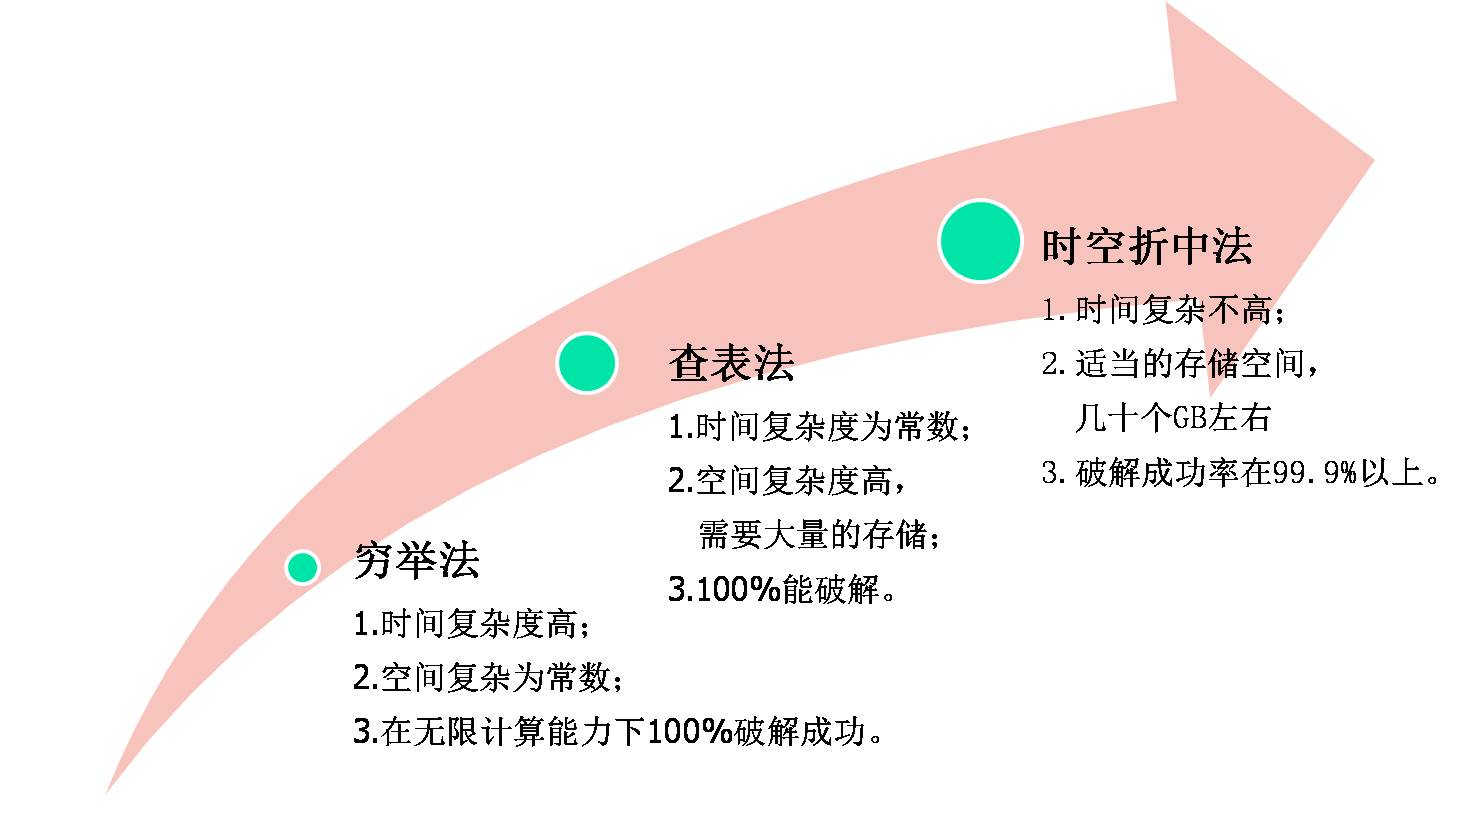
\includegraphics[scale=0.5]{2-1.jpg}
\caption{暴力攻击的几个方法比较}
\label{fig:2.1}
\end{figure}
\section{单向散列函数的破解}
\subsection{Hash函数的简介}
单向散列函数,又称单向Hash函数、杂凑函数,就是把任意长的输入消息串变化成固定长度的输出串的一种不可逆函数。这个输出串称为消息的散列值。一般用于密钥加密,产生消息摘要等。单向散列函数是现代密码学的一个重要领域,它是数据完整性检测、数字签名和认证方案中必不可少的一部分。单向Hash函数\cite{hash}是许多协议框架中的一个模块。目前由许多Hash函数的公开算法,一般一个安全的Hash函数应该至少满足以下几个条件:
\begin{enumerate}
\item 输入串值的长度是任意的;
\item 输出串Hash值长度是固定的;
\item 对每个给定的输入串的值,计算机得到输出Hash值是很容易的;
\item 给定Hash函数的描述,已知一个Hash值时,要找到输入串使它的的Hash值等于已知的这个Hash值在计算上时不可行的,或是找到两个不同的输入串,计算得到相同的输出Hash值在计算上是不可行的。
\end{enumerate}
Hash函数主要用于数据完整性校验和数字签名的有效性,常被用在身份认证上。例如在一个身份验证系统上,保存用户的密码时,需要把密钥用Hash算法进行加密,得到一个Hash值。由于Hash函数本身的特点,其他用户即使得到了这个Hash值也无法还原密码。当用户登录时,系统把用户输入的密码再用Hash算法进行计算,得到的Hash值与保存在系统中的Hash值进行比较,从而验证用户的合法性。
MD5\cite{md5}(Message-Digest Algorithm 5)是目前应用最广泛的 Hash 函数之一。MD5 将任意长度的“字节串”变换成一个 128比特的大整数,并且它是一个不可逆的字符串变换算法,换句话说就是,即使你看到源程序和算法描述,也无法将一个 MD5 的值变换回原始的字符串,从数学原理上说,是因为原始的字符串有无穷多个,这有点象不存在逆函数的数学函数。MD5在经过一些初始处理后,将明文分成了512位的块,再将每一块分成16个32位的子块。算法的输出是4个32位的块,连接起来就是128位的输出的Hash值。
\subsection{对Hash函数攻击的方法}
\begin{enumerate}
\item 替换法

这是一个十分实用的攻击方法,它并不对Hash算法本身作任何攻击,只是利用系统中的Hash函数重新生成一个Hash值,这个Hash值的输入串是攻击者已知的,如“password”,这样我们就可能把这串新生成的Hash值替换掉系统本身的Hash值,此时攻击者就能用“password”能登陆系统,从而达到绕过系统的认证机制。这种攻击方法需要攻击者已知目标系统认证机制使用的Hash算法函数(一般的系统都使用MD5算法函数)和由替换的权限。
\item 字典查表法

还有一种在实际破解中使用较多得方法是字典查询法,攻击者需要预先对目标Hash算法构造相应得字典文件,然后把需要破解得Hash值跟这个字典文件里得Hash值进行检索比较,通常这种办法需要TB级甚至跟大得存储空间,并且预运算的时间代价也是很大的。
\item 碰撞法

所谓杂凑碰撞指两个完全不同的讯息经杂凑函数计算得出完全相同的杂凑值。根据鸽巢原理,以有长度限制的杂凑函数计算没有长度限制的讯息是必然会有冲撞情况出现的。可是,一直以来,电脑保安专家都认为要任意制造出冲撞需时太长,在实际情况上不可能发生。2004年8月17日的美国加州圣巴巴拉的国际密码学会议(Crypto’2004)上,来自中国山东大学的王小云教授做了破译MD5、HAVAL-128、 MD4和RIPEMD算法的报告,公布了MD系列算法的破解结果。在破解MD5之后,2005年2月,王小云教授又破解了另一国际密码SHA-1,王小云的研究成果表明了从理论上讲电子签名可以伪造,必须及时添加限制条件,或者重新选用更为安全的密码标准,以保证电子商务的安全。2005年8月,王小云、姚期智,以及姚期智妻子姚储枫(即为Knuth起名高德纳的人)联手于国际密码讨论年会尾声部份提出SHA-1杂凑函数杂凑冲撞演算法的改良版。此改良版使破解SHA-1时间缩短。
\end{enumerate}
\section{本章小结}
本章简要介绍了密码分析学的发展背景、定义和研究的意义,重点阐述了现代密码分析的方法手段和密码攻击的类型,比较了暴力攻击法的几种方法,穷举法的虽然可以100\%破解成功,但这是建立在付出巨大的计算代价和时间代价;查表法则以巨大的存储代价来达到密码破解的目的;而时空折中法则是前两种办法的折中办法,以空间代价换取时间代价或者以时间代价换取空间代价,在两个中间找到一个平衡点,这样会损失一些破解成功率。最后以单向散列函数的破解为例,介绍了对Hash函数加密了的密钥的破解。

\chapter{时空折中算法}
本章主要要介绍时空折中算法的相关理论基础。从最初Martin Hellman的时空折中算法、Ronald Rivest的差异点DP方法到Philippe Oechslin在2003年基于前两种方法提出的彩虹表算法(RainBow Table),时空折中算法已经成为现代密码分析算法中一类极具现实意义的算法之一。这类算法一般都包括了以下两个主要步骤:1,预运算(pre-computation);2,在线分析(online phase)。本章节\ref{sec:3.1},\ref{sec:3.2}和\ref{sec:3.3}将分别介绍Martin Hellman表以及彩虹表的设计原理和构造思想。

我们将在本章中统一使用以下定义:N表示目标密码算法的密钥空间大小;T和M分别表示在线分析的时间代价以及预运算步骤所产生的密钥表空间大小;对于预运算的成功率P,我们通常认为分析者具有足够长的时间,所以该代价一般不作为讨论的内容并且将其粗略等价于穷举所有密钥表空间的时间。
\section{Martin Hellman最初的算法}
\label{sec:3.1}
Martin Hellman在1980年第一次提出基于时间空间折中算法的分组密码算法DES的密码分析\cite{hellman}。攻击者使用的是选择明文攻击,也就是给定一个指定的明文加密后的密文,尝试从密文中分析恢复出这次加密的密钥。因此攻击者所要关心的问题是如何从N中找出对应的密钥,以56比特DES为例,其密钥空间为$N=2^{56}$。(若无特殊说明,下文都将以56比特的DES为目标密码算法)
	\subsection{预运算}
在预运算阶段,算法将首先固定一个目标密文所对应的明文P,一般大小为8个字符(64比特),接着结合P构造如下非逆函数f:
\begin{equation}f(k)=R(S_k(P))
\label{equ:3_1}
\end{equation}
其中P是所选的固定明文信息,S表示伪随机函数,R是一个从密文空间到密文空间的简约(Reduction)函数,并且在下文令S=DES。对于R函数的选择,若无特别说明,我们将假定任一从64比特到56比特的映射函数均可适用。通常为了简便起见,令R函数为仅简单地地去掉64比特的高8位。从而R、S复合而成的f函数可以看作是一个56比特到56比特的伪随机函数。

预运算开始时,算法将选择m个来自密钥空间N的随机密钥作为开始节点(Start Point,简称SP),令其为$SP_1,SP_2,SP_3\ldots SP_{m-1},SP_m$。接着,将$SP_1$作为输入代入公式\eqref{equ:3_1},并迭代t次,得到如下两式\eqref{equ:3_2}和\eqref{equ:3_3}:
\begin{equation}k_i=f(k_{i-1})  (1\leq i \leq t)
\label{equ:3_2}
\end{equation}
\begin{equation}SP_1=k_{10}\xlongrightarrow{f} k_{11}\xlongrightarrow{f} k_{12}\xlongrightarrow{f}\cdots \xlongrightarrow{f} k_{1t}=EP_1
\label{equ:3_3}
\end{equation}

其中,令结束节点(End Point,简称EP)$EP=f(K_{t-1})$。当每个$SP_j$都完成t次迭代后,我们就会得到一张有m对形式如$(SP_j,EP_j) (1\leq j \leq m)$的二元组构成的Hellman表。
\begin{equation}
\underbrace{\begin{bmatrix}
SP_1=k_{10}\xlongrightarrow{f} k_{11}\xlongrightarrow{f} k_{12}\xlongrightarrow{f}\cdots \xlongrightarrow{f} k_{1t}=EP_1 \\
SP_2=k_{20}\xlongrightarrow{f} k_{21}\xlongrightarrow{f} k_{22}\xlongrightarrow{f}\cdots \xlongrightarrow{f} k_{2t}=EP_2 \\
\vdots \\
SP_m=k_{m0}\xlongrightarrow{f} k_{m1}\xlongrightarrow{f} k_{m2}\xlongrightarrow{f}\cdots \xlongrightarrow{f} k_{mt}=EP_m \\
\end{bmatrix}}_{\text{迭代}t\text{次}}
\end{equation}
\begin{equation}
\begin{bmatrix}
SP_1 & EP_1 \\
SP_2 & EP_2 \\
\vdots & \vdots \\
SP_m & EP_m
\end{bmatrix}
\label{equ:3.8}
\end{equation}
这里要注意的是,在SP和EP之间的节点都不会被保存,如\eqref{equ:3.8}式。这些值可以依靠相应的二元组在需要使用的时候可以在线计算生成,这也就是把节省了空间,而关于m,t的选择,就是这个时间于空间折中的选择,一般它们应当满足:
\begin{equation}mt^2=N
\label{equ:3.4}
\end{equation}
而且\eqref{equ:3.4}式也被成为矩阵终止规则(Matrix stopping rule)。根据生日悖论思想,当上式成立时,将不会有太多的重复节点出现,而当m或t过大使得$mt^2>N$,则冲突数量将快速上升,并最后导致Hellman表的成功率下降。而事实上,在实际的密钥攻击过程中,可以允许$mt^2<N$,只不过相应的攻击成功率会有所下降。
	\subsection{在线分析阶段}
        \label{sec:3.1.2}
在线分析阶段,给定已知明文P和对应的密文C,代入R(C)可以得到$y_1$,然后将$y_1$与$EP_i(i=1,2,\ldots ,m)$比较,若存在某个i,使得等式$y_i=EP_i$成立,则会出现以下两种情况:1,加密$y_1$的密钥为$K=k_{i,t-1}$;2,所对应的密钥不在表中,这个现象叫做False alarm。 若等式$y_1=EP_i$不成立,则继续迭代下一步$y_2=f(y_1)$,并重复上一步相同的比较,直到出现以下三种情况:1,找到密钥;2,出现False alarm,就也就假警;3,表搜索结束。简单地讲,在线分析的目的是在Hellman表中搜索出正确的密钥K,使得$K=k_{ij}=y_{t-j}$。需要注意的是,在线分析过程中的$y_j$是可以反复利用与$y_{j+1}$计算的,之后介绍的彩虹表将无法重用。
	\subsection{TMTO曲线}
在介绍TMTO曲线前,我们将先讨论Hellman表的空间代价和时间代价。在忽略二元组$(SP_j,EP_j)$本身大小和一些其他较小的常量后,我们可以计算出存储t张维度为$m	imes t$大小的Hellman表需要的空间M=mt。同时,由于试图要覆盖整个密钥空间,故预运算的代价P=N。在线分析阶段,每一张表的搜索,函数f最多会被调用t次,因此t张表的总时间代价$T=t^2$,由于搜索的代价相对比较低,在这里可以忽略不计。基于上述时间和空间的代价分析就很容易得到TMTO曲线:
\begin{equation}TM^2=N^2\text{并且} P=N
\label{equ:3.5}
\end{equation}
反之,当给定时间代价T和空间代价M时,则可以通过3.5式推出m和t,也就是说可以在时间T和空间M得限制下,从以m,t为参数得Hellman表中找到正确得密钥K。

结合\eqref{equ:3.4}式和\eqref{equ:3.5}式我们得到一个重要的等式:
\begin{equation}T=M=N^{\tfrac{2}{3}}
\label{equ:3.6}
\end{equation}
由等式\eqref{equ:3.6}可知,密码分析者在使用Hellman表来成功破解密钥K所需要的代价会比穷举攻击快$N^{\tfrac{1}{3}}$倍,当然前提都是在基于选择明文的攻击方式下。由伪随机函数S的特性可以得到,只要稍加修改,比如将函数R的输入输出长度改变,我们就能对其他的分组密码算法进行密钥破解。所以,对任意的密钥空间为N的分组密码,利用Hellman算法都能获得以$N^{\tfrac{2}{3}}$为代价的密钥破解成功。而针对其他体制的加密算法的密钥分析,例如以杂凑Hash函数为代表的MD5和SHA-1的加密算法,我们将在下面的彩虹表讨论分析。
	\subsection{密钥分析的成功率}
在上一章\ref{sec:2.4}节密码分析方法的比较中,我们已经得出了相对穷举法百分之百的破解成功率来说,Hellman的时空折中算法并非是100\%能破解成功的,即使你付出了$N^{\tfrac{2}{3}}$的代价。换句话说,也就是这类的时空折中算法是以牺牲少量的成功率为代价换取了在时间或空间上的代价,这也充分体现了折中的这个思想。因此,本节将会重点分析Hellman算法的成功率。其实造成功率损失的根本原因在与算法本身,由于简约函数R仅是从密文空间V到密钥空间N的这么一个映射,而对于两个不同的密文$C_1$,$C_2$,会有一定概率映射到同一个密文,并造成Hellman表中的节点因发生了碰撞而不唯一,如图\ref{fig:3.1}所示,因此导致了最终的破解成功率降低。一般来说,当m,t值越大,节点间发生碰撞合并的概率也就越高。并且由于Hellman表的每个节点都使用相同的R函数,所以一旦表中任意两个节点发生碰撞时,这两个节点之后的所有节点也将会发生碰撞,最坏的情况会导致50\%的效率下降。
\begin{figure}[!ht]
\centering
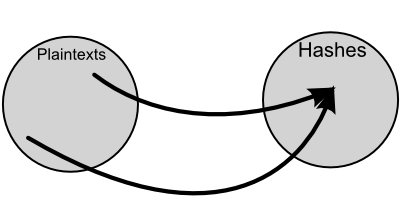
\includegraphics{collision.png}
\caption{碰撞示意图}
\label{fig:3.1}
\end{figure}

成功率是随着m,t的增大非线性地提升。在文献\cite{hellman}中,我们可以得知一张m行,t列的Hellman表能成功破解密钥K的概率公式为:
\begin{equation}
P_{Hellman}\geq \frac{1}{N}\sum_{i=1}^{m}\sum_{j=0}^{t-1}\left(1-\frac{it}{N}\right)^{j+1}
\label{equ:3.7}
\end{equation}
由于有节点的碰撞,单表的破解成功概率会随着表的大小增大而放缓增幅,所以为了得到更高的破解成功概率,我们一般都会使用多张表,例如\eqref{equ:3.4}式中的t张表,并且为了避免表与表之间的链碰撞合并,不同的表当中应当使用不同的函数$R_j(1\leq j \leq t)$使得即使不同表间两个节点相同也难导致链表的合并。因此,我们也就很容易得到了t张Hellman表的总成功率公式:
\begin{equation}
\boxed{P_{Hellman}^{All}\geq 1-\left(1-\frac{1}{N}\sum_{i=1}^{m}\sum_{j=0}^{t-1}\left(1-\frac{it}{N}\right)^{j+1}\right)^t}
\end{equation}
Hellman称上述节点发生碰撞导致链合并的现象为False Alarm,也就是出现了上文\ref{sec:3.1.2}提到的有$y_k=EP_i$,但对应的$k_{i,t-k}$不等于正确密钥。直观上分析,表的规模越大,越有概率发生假警,若假警率过高,则在线分析会花费大量的代价在剔除假警,为此Hellman给出了一个假警上界:
\begin{equation}
E(F)\leq \frac{mt(t+1)}{2N}
\end{equation}
当假警发生时,最坏情况时导致t次函数f的迭代开销,也就是在一开始发生了假警,此时这个代价等同与在线分析时计算$y_1,y_2\ldots y_t$的代价。因此当有$mt^2=N$,且$N\guillemotright 1$时,有$E(F)\leq \frac{1}{2}$,则由于总的开销最多为$\frac{t}{2}$次迭代,从而可以保持假警代价不超过$\frac{t^2}{2}$,即$\frac{T}{2}$。
\section{Ronald Rivest差异点DP方法}
\label{sec:3.2}
在随后的1982年,Ronald Rivest提出了差异点(DP)的概念,通过使用差异点减少对磁盘的访问次数,有效地解决了碰撞的问题,从而降低破解的代价。差异点式满足一套标准的数据点。我们定义密钥的前10比特为一个特定的二进制,为了简便起见,这里设定为零。Rivest提出只存储差异点作为终点,在破解密文时,简单地根据Hellman的方法生成链直到发现一个差异点,当且仅当发现一个差异点时,才在表中进行查找,这可以大大提升算法的性能。

差异点自提出后就被广泛地研究和使用,在1982年和2003年间这一领域的大多数研究都是基于差异点的。Koji Kusuda和Tsutomu Matsumoto\cite{koji}一文中具体讨论了如何提升破解的成功率,通过研究证明调整表中的参数可以降低内存的消耗,以获得更高的成功率,更快地破解密钥。另外,Johan Borst,Bart Preneel和Joos Vandewalle\cite{jbj}共同发表的一篇文献中也对差异点进行了研究,他们介绍了一种分布式的密钥搜索算法,在基于Hellman的假设,认为存储访问代价时微不足道的,研究表明执行分布式密钥搜索时,这个假设不再合理,他们还提出一种可大大减少内存访问次数的折中算法,从而减少与分布式密钥搜索相关的问题。然而,他们的研究在1998年完成,这就意味着他们的工作与2003年Oechslin的工作毫无关联,分布式密钥搜索也与实际的表的生成无关,下面我们将重点介绍Philippe Oechslin在2003年改进后的算法,也就是目前著名的彩虹表算法。
\section{Philippe Oechslin的彩虹表算法}
\label{sec:3.3}
	\subsection{非完美彩虹表}
如\ref{sec:3.1}节所述,Hellman表的一个主要不足是表大小的限制,当以增大表大小来获得更高得成功率时,表中的节点碰撞而导致的链合并概率也会随之增加,且增加的比例同m与t的平方成正比。为了解决这一不足,在2003年,Oechslin在Hellman算法的基础上结合了Rivest的差异点(DP)的优势,提出了一种在当时比较先进的算法--彩虹表算法\cite{PO}。通过这种时空折中算法预运算所生成的表,我们称之为彩虹表(Rainbow Table),彩虹表中的行称为彩虹链。

与Hellman算法在一张表中只使用一个f函数不同,彩虹表的每一列使用的R函数都不一样,以构造不同的f函数,如式\eqref{equ:3.10}所示:
\begin{equation}
\label{equ:3.10}
f_i(k)=R_i(S_k(P)) \quad \quad  (1\leq i \leq t) 
\end{equation}
从上式可以看出,彩虹表用$R_1,R_2,\ldots ,R_t$代替Hellman表中的R函数。因此,只有在当彩虹表中两个节点在同一列发生碰撞时,才会发生链合并。换句话说,如果碰撞发生在不同列的两个节点,由于不同列采用的不同的R函数,碰撞点之后的链不会被合并。

我们假设一张彩虹表有m条彩虹链,每条彩虹链的长度为t,即为$m\times t$的矩阵,如式\eqref{equ:3.11}:
\begin{equation}
\label{equ:3.11}
\begin{bmatrix}
k_{1,1} & k_{1,2} & \cdots & k_{1,t-1} & k_{1,t} \\
k_{2,1} & k_{2,2} & \cdots & k_{2,t-1} & k_{2,t} \\
\vdots & \vdots & \vdots & \vdots & \vdots \\
k_{m,1} & k_{m,2} & \cdots & k_{m,t-1} & k_{m,t} \\
\end{bmatrix}
\end{equation}
现在来计算这张彩虹表的破解成功率P,这个问题实质上等价与整个矩阵每列的概率乘积。第一个元素$k_{1,1}$命中的概率为$\frac{1}{N}$,那么这一列命中概率为$P_1=\frac{m_{1}}{N}$;则第二列命中的概率为$P_2=1-(1-\frac{1}{N})^{m_1}$,当$N\gg m_{1}$时,$P_2=1-e^{-\tfrac{m_1}N{}}$,因此,可以得到第i列的命中概率公式:
\begin{equation}
P_i=1-e^{-\tfrac{m_{i-1}}{N}}=\frac{m_i}{N}
\end{equation}
在概率定理可以推出整张彩虹表的成功率公式为:
\begin{eqnarray}
\label{equ:3.12}
P_{Rainbow} \ge 1-\prod^{t}_{i=1}\left(1-\frac{m_{i}}{N}\right) \nonumber\\
\text{其中,} m_{1}=m \text{,且} m_{n+1} = N\left(1-e^{-\tfrac{m_{n}}{N}}\right)
\end{eqnarray}

比较\eqref{equ:3.7}式和\eqref{equ:3.12}式,我们可以发现t张$m\times t$Hellman表与1张$mt\times t$的彩虹表有大致相同的成功率。因为这两种算法所产生的表都覆盖了$mt^2$的密钥空间,同时也都包含了t个不同的R函数。在假警方面,两者也有类似的共同点,单张彩虹表的一列以及t张Hellman表,若包含mt个节点,则这些节点中的任一碰撞都将会导致链的合并。
在线分析过程中,彩虹表算法的搜索过程与Hellman算法有所不同,首先,将给定的密文C代入$R_t$的$y_1$,并检索是否存在某个$EP_i=y_1$,如果找到了匹配的$EP_i$,这可以通过保存的对应$SP_i$来恢复$k_{t,t-1}$。若找不到匹配的EP,则将密文C依次代入$R_{t-1}$,再次搜索判断是否存在正确的密钥在第t-2列中。以此类推,最坏的情况下将遍历表中所有的t列,以f函数迭代次数为标准,这个代价为$1+2+\cdots +(t-1)=\frac{t(t-1)}{2}$次。而Hellman表需要搜索$t^2$次,因而单张的彩虹表相比t张Hellman表,搜索代价只有不到Hellman算法的一半。
	
在此小结一下彩虹表相对Hellman表的优点:\\
1),从搜索次数角度来看,彩虹表最多需要比较$log(mt)*t$次,而Hellman表将最多需要$log(t)*t^2$,即搜索t表t列。因此彩虹表的比较次数约为Hellman的$\frac{1}{t}$,彩虹表相应的TMTO曲线为:
\begin{equation}
TM^2=\frac{1}{2}N^2
\end{equation}
2),彩虹表中若发生彩虹链合并时,则会导致对应的EP点相同。当需要构造没有重复链的完美表(Perfect Table)时,可以通过检查EPs来完成。而Hellman表则无此特性。需要注意的是在完美表中并不是没有碰撞节点,而是碰撞节点不在同一列上出现。\\
3),由于彩虹链中的t个R函数均不相同,因此链中将几乎不会产生循环。以Hellman链为例,若同一链中出现了两个节点$k_i,k_j$,使得$k_i=k_j$,那么由于该链使用相同的R函数,故从这两个相同节点的后面节点都会相等,依次类推,最多会导致j-i个节点的重复,进而缩小了整个Hellman表的覆盖率。该现象不会产生假警,然而会降低成功率。而彩虹表则没有相应的问题。\\
4),与Hellman表的变形差异点(DP)算法相比,彩虹表的链条长度是固定的,这个特性对彩虹表的程序代码实现是十分有利的,同时也会使得假警率有所下降,从而提高了成功率。
	\subsection{完美彩虹表}
当表中出现合并链时,彩虹表和差异点DP算法都可以通过检查是否具有相同的EP节点方式来检测出合并,而通常情况在预运算后生成的表需要排序的,这样一来就可以很容易地从表中剔除重复的链,而经过剔除重复链后的表我们称之为完美彩虹表。特别是在当内存空间有限时,我们总希望表能包含尽可能多的唯一节点,以提高成功率。生成相对应的Hellman完美表,则不得不搜索整张表,每个节点均要O(mt)次搜索,显然这是不现实的。在完美彩虹表中,有$m_i=m_1=m (2\leq i \leq t)$,因此成功率可化简为:
\begin{equation}
\label{equ:3.13}
P_{perfect}=1-\prod^{t}_{i=1}\left(1-\frac{m}{N}\right)
\end{equation}

从\eqref{equ:3.13}式可知,成功率直接与完美彩虹表的初始参数m,t有关,也就是表越大,成功率$P_{perfect}$应越大。同时与非完美彩虹表比较,不但减少了因存储重复节点而造成的空间浪费,而且节省了在线分析的时间代价。对于一个给定的t,假设选择$m_1=N$时得到的$m_t \text 为 m_{max}(t)$,表示为完美彩虹表最大的独立结束节点EPs的个数,其中$m_{i+1}=N\left(1-e^{-\tfrac{m_i}{N}}\right)(1\leq i \leq t)$。

当$t\gg 1$时,利用泰勒公式可以得到\cite{aa}:
\begin{equation}
m_{max}(t)\approx \dfrac{2N}{t+2}
\end{equation}
将上式代入\eqref{equ:3.13}式便可得出完美彩虹表成功率的最大期望值为:
\begin{equation}
P_{perfect}^{max}=1-\left(1-\dfrac{m_{max}}{N}\right)^t \approx 1-e^{-t\tfrac{m_{max}}{N}} \approx 1-e^{-2} \approx 86\%
\end{equation}
也就是说,对于N和较大的t,完美彩虹表的成功率会随着m,t的增大而趋于一个常量。因此,单张的彩虹表的成功率要小于80\%,若要较高的成功率P$(P>90\%)$,则可以通过多张彩虹表来实现。
\section{本章小结}
本章主要简要地介绍了3种典型的时空折中算法,包括Hellman算法、差异点DP算法和彩虹表算法。时空折中算法主要包括预运算和在线分析两个步骤。Hellman表和彩虹表具有不同的折中曲线,分别式$TM^2=N^2$和$TM^2=\frac{1}{2}N^2$。重点分析了彩虹表的成功率,包括公式的推导演算和证明。



\chapter{彩虹表算法的实现}
\section{彩虹表的算法分析}
\label{sec:3.3}
	\subsection{非完美彩虹表}
如\ref{sec:3.1}节所述,Hellman表的一个主要不足是表大小的限制,当以增大表大小来获得更高得成功率时,表中的节点碰撞而导致的链合并概率也会随之增加,且增加的比例同m与t的平方成正比。为了解决这一不足,在2003年,Oechslin在Hellman算法的基础上结合了Rivest的差异点(DP)的优势,提出了一种在当时比较先进的算法--彩虹表算法\cite{PO}。通过这种时空折中算法预运算所生成的表,我们称之为彩虹表(Rainbow Table),彩虹表中的行称为彩虹链。
与Hellman算法在一张表中只使用一个f函数不同,彩虹表的每一列使用的R函数都不一样,以构造不同的f函数,如式\eqref{equ:3.10}所示:
\begin{equation}
\label{equ:3.10}
f_i(k)=R_i(S_k(P)) \quad \quad  (1\leq i \leq t) 
\end{equation}
从上式可以看出,彩虹表用$R_1,R_2,\ldots ,R_t$代替Hellman表中的R函数。因此,只有在当彩虹表中两个节点在同一列发生碰撞时,才会发生链合并。换句话说,如果碰撞发生在不同列的两个节点,由于不同列采用的不同的R函数,碰撞点之后的链不会被合并。
我们假设一张彩虹表有m条彩虹链,每条彩虹链的长度为t,即为$m\times t$的矩阵,如式\eqref{equ:3.11}:
\begin{equation}
\label{equ:3.11}
\begin{bmatrix}
k_{1,1} & k_{1,2} & \cdots & k_{1,t-1} & k_{1,t} \\
k_{2,1} & k_{2,2} & \cdots & k_{2,t-1} & k_{2,t} \\
\vdots & \vdots & \vdots & \vdots & \vdots \\
k_{m,1} & k_{m,2} & \cdots & k_{m,t-1} & k_{m,t} \\
\end{bmatrix}
\end{equation}
现在来计算这张彩虹表的破解成功率P,这个问题实质上等价与整个矩阵每列的概率乘积。第一个元素$k_{1,1}$命中的概率为$\frac{1}{N}$,那么这一列命中概率为$P_1=\frac{m_{1}}{N}$;则第二列命中的概率为$P_2=1-(1-\frac{1}{N})^{m_1}$,当$N\gg m_{1}$时,$P_2=1-e^{-\tfrac{m_1}N{}}$,因此,可以得到第i列的命中概率公式:
\begin{equation}
P_i=1-e^{-\tfrac{m_{i-1}}{N}}=\frac{m_i}{N}
\end{equation}
在概率定理可以推出整张彩虹表的成功率公式为:
\begin{eqnarray}
\label{equ:3.12}
P_{Rainbow} \ge 1-\prod^{t}_{i=1}\left(1-\frac{m_{i}}{N}\right) \nonumber\\
\text{其中,} m_{1}=m \text{,且} m_{n+1} = N\left(1-e^{-\tfrac{m_{n}}{N}}\right)
\end{eqnarray}

比较\eqref{equ:3.7}式和\eqref{equ:3.12}式,我们可以发现t张$m\times t$Hellman表与1张$mt\times t$的彩虹表有大致相同的成功率。因为这两种算法所产生的表都覆盖了$mt^2$的密钥空间,同时也都包含了t个不同的R函数。在假警方面,两者也有类似的共同点,单张彩虹表的一列以及t张Hellman表,若包含mt个节点,则这些节点中的任一碰撞都将会导致链的合并。
上述这样等规模的Hellman表和彩虹表的比较可以参考式\eqref{equ:3.20}
\begin{gather}
\label{equ:3.20}
\begin{bmatrix}
k_{1,0}^1\xlongrightarrow{f_1} k_{1,1}^1\xlongrightarrow{f_1} \cdots \xlongrightarrow{f_1}k_{1,t}^1 \\
\vdots \\
k_{m,0}^1\xlongrightarrow{f_1} k_{m,1}^1\xlongrightarrow{f_1} \cdots \xlongrightarrow{f_1}k_{m,t}^1 \\
\end{bmatrix} \\ 
\begin{bmatrix}
k_{1,0}^t\xlongrightarrow{f_t} k_{1,1}^t\xlongrightarrow{f_t} \cdots \xlongrightarrow{f_t}k_{1,t}^t \\
\vdots \\
k_{m,0}^t\xlongrightarrow{f_t} k_{m,1}^t\xlongrightarrow{f_t} \cdots \xlongrightarrow{f_t}k_{m,t}^t \\
\end{bmatrix}\\
\begin{bmatrix}
k_{1,0}^1\xlongrightarrow{f_1} k_{1,1}^1\xlongrightarrow{f_2} \cdots \xlongrightarrow{f_t}k_{1,t}^1 \\
k_{2,0}^1\xlongrightarrow{f_1} k_{1,1}^1\xlongrightarrow{f_2} \cdots \xlongrightarrow{f_t}k_{2,t}^1 \\
\cdots \\ 
\\ \\
\cdots \\
k_{mt-1,0}^1\xlongrightarrow{f_1} k_{1,1}^1\xlongrightarrow{f_2} \cdots \xlongrightarrow{f_t}k_{mt-1,t}^1 \\
k_{mt,0}^1\xlongrightarrow{f_1} k_{1,1}^1\xlongrightarrow{f_2} \cdots \xlongrightarrow{f_t}k_{mt,t}^1
\end{bmatrix}
\end{gather}
在线分析过程中,彩虹表算法的搜索过程与Hellman算法有所不同,首先,将给定的密文C代入$R_t$的$y_1$,并检索是否存在某个$EP_i=y_1$,如果找到了匹配的$EP_i$,这可以通过保存的对应$SP_i$来恢复$k_{t,t-1}$。若找不到匹配的EP,则将密文C依次代入$R_{t-1}$,再次搜索判断是否存在正确的密钥在第t-2列中。以此类推,最坏的情况下将遍历表中所有的t列,以f函数迭代次数为标准,这个代价为$1+2+\cdots +(t-1)=\frac{t(t-1)}{2}$次。而Hellman表需要搜索$t^2$次,因而单张的彩虹表相比t张Hellman表,搜索代价只有不到Hellman算法的一半。

在此小结一下彩虹表相对Hellman表的优点:\\
1),从搜索次数角度来看,彩虹表最多需要比较$log(mt)*t$次,而Hellman表将最多需要$log(t)*t^2$,即搜索t表t列。因此彩虹表的比较次数约为Hellman的$\frac{1}{t}$,彩虹表相应的TMTO曲线为:
\begin{equation}
TM^2=\frac{1}{2}N^2
\end{equation}
2),彩虹表中若发生彩虹链合并时,则会导致对应的EP点相同。当需要构造没有重复链的完美表(Perfect Table)时,可以通过检查EPs来完成。而Hellman表则无此特性。需要注意的是在完美表中并不是没有碰撞节点,而是碰撞节点不在同一列上出现。\\
3),由于彩虹链中的t个R函数均不相同,因此链中将几乎不会产生循环。以Hellman链为例,若同一链中出现了两个节点$k_i,k_j$,使得$k_i=k_j$,那么由于该链使用相同的R函数,故从这两个相同节点的后面节点都会相等,依次类推,最多会导致j-i个节点的重复,进而缩小了整个Hellman表的覆盖率。该现象不会产生假警,然而会降低成功率。而彩虹表则没有相应的问题。\\
4),与Hellman表的变形差异点(DP)算法相比,彩虹表的链条长度是固定的,这个特性对彩虹表的程序代码实现是十分有利的,同时也会使得假警率有所下降,从而提高了成功率。
	\subsection{完美彩虹表}
当表中出现合并链时,彩虹表和差异点DP算法都可以通过检查是否具有相同的EP节点方式来检测出合并,而通常情况在预运算后生成的表需要排序的,这样一来就可以很容易地从表中剔除重复的链,而经过剔除重复链后的表我们称之为完美彩虹表。特别是在当内存空间有限时,我们总希望表能包含尽可能多的唯一节点,以提高成功率。生成相对应的Hellman完美表,则不得不搜索整张表,每个节点均要O(mt)次搜索,显然这是不现实的。在完美彩虹表中,有$m_i=m_1=m (2\leq i \leq t)$,因此成功率可化简为:
\begin{equation}
\label{equ:3.13}
P_{perfect}=1-\prod^{t}_{i=1}\left(1-\frac{m}{N}\right)
\end{equation}

从\eqref{equ:3.13}式可知,成功率直接与完美彩虹表的初始参数m,t有关,也就是表越大,成功率$P_{perfect}$应越大。同时与非完美彩虹表比较,不但减少了因存储重复节点而造成的空间浪费,而且节省了在线分析的时间代价。对于一个给定的t,假设选择$m_1=N$时得到的$m_t \text 为 m_{max}(t)$,表示为完美彩虹表最大的独立结束节点EPs的个数,其中$m_{i+1}=N\left(1-e^{-\tfrac{m_i}{N}}\right)(1\leq i \leq t)$。

当$t\gg 1$时,利用泰勒公式可以得到\cite{aa}:
\begin{equation}
m_{max}(t)\approx \dfrac{2N}{t+2}
\end{equation}
将上式代入\eqref{equ:3.13}式便可得出完美彩虹表成功率的最大期望值为:
\begin{equation}
P_{perfect}^{max}=1-\left(1-\dfrac{m_{max}}{N}\right)^t \approx 1-e^{-t\tfrac{m_{max}}{N}} \approx 1-e^{-2} \approx 86\%
\end{equation}
也就是说,对于N和较大的t,完美彩虹表的成功率会随着m,t的增大而趋于一个常量。因此,单张的彩虹表的成功率要小于80\%,若要较高的成功率P$(P>90\%)$,则可以通过多张彩虹表来实现。

\section{彩虹表的构建与产生}
\subsection{定义Hash函数}
本文的实现了对SHA-1、MD5和LM三种Hash函数的破解,下面代码对LM算法的实现:
\begin{lstlisting}
void HashLM(unsigned char* pPlain, int nPlainLen, unsigned char* pHash)
{   
  int i; 
  for (i = nPlainLen; i < 7; i++)
  pPlain[i] = 0;
  static unsigned char magic[] = {0x4B, 0x47, 0x53, 0x21, 0x40, 0x23, 
                                                            0x24, 0x25};
  des_key_schedule ks;
  setup_des_key(pPlain, ks);
  des_ecb_encrypt((des_cblock*)magic,(des_cblock*)pHash,ks,DES_ENCRYPT);
}
\end{lstlisting}
SHA1和MD5函数的实现则是调用了OpenSSL的API函数:
\begin{lstlisting}
unsigned char *MD5(const unsigned char *d, size_t n, unsigned char *md);
\end{lstlisting}
\begin{lstlisting}
unsigned char *SHA1(const unsigned char *d, size_t n, unsigned char *md);
\end{lstlisting}
\subsection{定义Reduce函数}
\subsection{彩虹表参数}
\subsection{构建彩虹表}
彩虹表算法实现的首要事情就是要产生符合自己需求的彩虹表文件,本次实现要求彩虹表的破解成功率在99.9%以上。

彩虹表算法中有许多参数变量,在构造一张彩虹表前必须先弄明白每个参数的含义,在这里我们为了方便下文叙述,统一给出彩虹表算法中会出现的参数和变量:Hash计算能力,取决于CPU和GPU等硬件设备;硬盘读写速度,取决于硬盘;密钥空间N;
\begin{enumerate}
\item 每条彩虹链的长度t;
\item 一张彩虹表中彩虹链的个数m;
\item 彩虹表的个数L;
\item 磁盘占用量M\quad 彩虹表所占用的存储空间;
\item 破解成功率P\quad 破解密钥的成功概率;
\item 破解时间;
\item 预运算时间;
\end{enumerate}
由上述可知,一张彩虹表是由许多彩虹链组成的,每个彩虹链在程序中的数据结构如下:\\
\begin{lstlisting}
struct RainbowChain 
{
	unit64 nIndexS;		//链表的初始元素
	unit64 nIndexE;		//链表的末尾元素
}
\end{lstlisting}
函数主要输入参数:
\begin{lstlisting}
	string sHashRoutineName  = argv[1];	
	//需要破解的算法名称
	string sCharsetName      = argv[2];				
	int nPlainLenMin         = atoi(argv[3]);
	//密码长度最小值
	int nPlainLenMax         = atoi(argv[4]);
	//密码长度最大值
	int nRainbowTableIndex   = atoi(argv[5]);			
	int nRainbowChainLen     = atoi(argv[6]);			
	int nRainbowChainCount   = atoi(argv[7]);			
\end{lstlisting}
生成彩虹表的关键代码:
\begin{lstlisting}
	int i;
	for (i = nDataLen / 16; i < nRainbowChainCount; i++) 
	{
		cwc.GenerateRandomIndex();
		uint64 nIndex = cwc.GetIndex();
		int nPos;
		for (nPos = 0; nPos < nRainbowChainLen - 1; nPos++)
		{
			cwc.IndexToPlain();
			cwc.PlainToHash();
			cwc.HashToIndex(nPos);		//缩减函数
		}
		nIndex = cwc.GetIndex();

\end{lstlisting}

初始节点nIndexS由cwc.GenerateRandomIndex()函数随机产生,并把当前的index值也赋予CChainWalkContext.m\_nIndex中, m\_nindex起到中间记录作用,当经过nRainbowChainLen(参数t)次循环计算得到nIndexE。

彩虹表生成算法描述:
\begin{enumerate}
\item 将随机生成的nIndexS通过函数cwc.IndexToPlain()转化成明文Plain,这一转化过程与二进制转16进制差不多,只是根据明文字符集长度(m\_nPlainCharsetLen)来变化;
\item 对步骤1生成的Plain进行Hash函数计算,通过PlainToHash()函数实现;
\item 对步骤2生成的Hash值进行缩减运算,缩减函数为HashToIndex(nPos),最后得到的nIndex必须在预设的字符空间范围内。
\end{enumerate}

将以上三步循环nRainBowChainLen次数后,我们将得到nIndexE和彩虹链的长度,当生成了m条彩虹链之后,这些彩虹链所组合起来的就是一张彩虹表文件。由于在循环过程中所产生的index只保存在内存里,并不写入磁盘文件,但是我们依然可以通过初始的Index计算出这过程中所有的index值。
\begin{equation}
\label{equ:4.1}
\begin{bmatrix}
Index\_Start_1 & Index\_End_1 \\
Index\_Start_2 & Index\_End_2 \\
\vdots  & \vdots \\
Index\_Start_m & Index\_End_m 
\end{bmatrix}
\end{equation}
从彩虹表的结构\eqref{equ:4.1}我们可以很容易得知一个彩虹链的所占的磁盘空间为$2*64=128$比特,也就是16Byte。由此得到彩虹表磁盘空间占用公式:
\begin{equation}
\label{equ:4.2}
M=16*m*l
\end{equation}
其中m为彩虹链的条数,l为彩虹表的个数。图\ref{fig:4.1}为彩虹表生成程序,hash\_algorithm 为目标密码hash算法;charset为密钥的字符集,决定这张彩虹表的密钥空间;还有链表长度和链表个数等参数。
\begin{figure}[!ht]
\centering
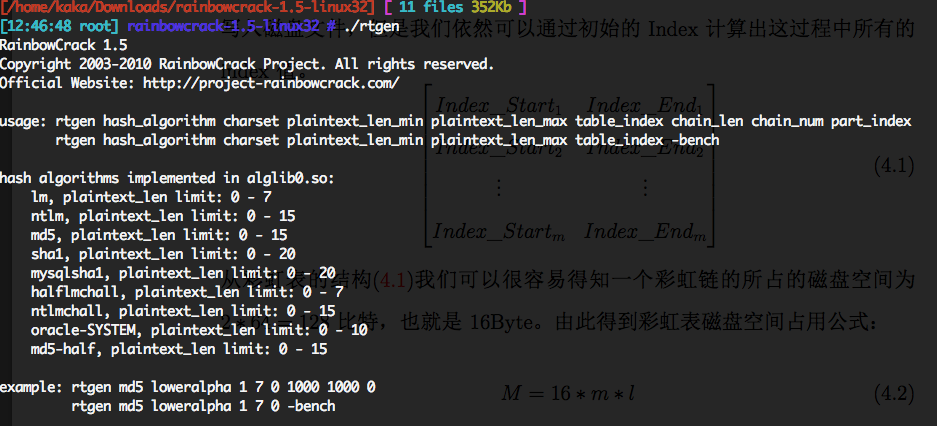
\includegraphics[scale=0.4]{4-1.png}
\caption{彩虹表生成程序}
\label{fig:4.1}
\end{figure}
\begin{figure}[!ht]
\centering
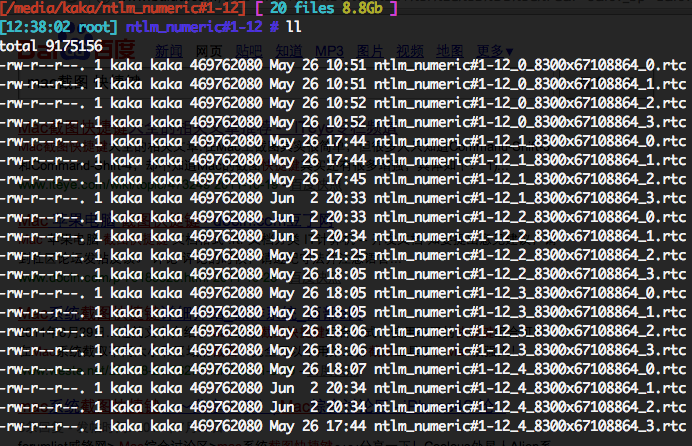
\includegraphics[scale=0.5]{4-2.png}
\caption{ntlm算法彩虹表}
\label{fig:4.2}
\end{figure}
从图\ref{fig:4.2}中我们可以看到20张彩虹表,hash\_algorithm为ntlm算法,ntlm为Windows NT系统的用户登陆验证算法;密钥字符集为numeric,也就是0~9,最小长度为1,最大长度为12,因此这个密钥空间$N=10^{12}+10^{11}+ \cdots +10^2 +10$,其他的密钥并不在这20张表里,一定不会被搜索到,想要破解需要加大链的数目,或者链表长度,或者表的张数;链表长度为8300,链表个数为67108864,这样通过公式\eqref{equ:4.2}我们很容易到这20张表的所占用的磁盘空间$M=20GB$,每张表的大小为1GB。
\section{密钥破解}
\subsection{搜索算法}
用彩虹表进行破解的过程其实质就是对彩虹表文件进行整表搜索的过程,简单来讲就是查表。破解的成功率和破解的时间基本上由预运算所生成的彩虹表决定,生成优质的彩虹表对破解的效率影响很大。具体的优化方法和技巧我们将在下文详细介绍,这一节我们要讨论的是彩虹表如果进行查表破解。首先我们看图\ref{fig:4.3}:
\begin{figure}[!ht]
\centering
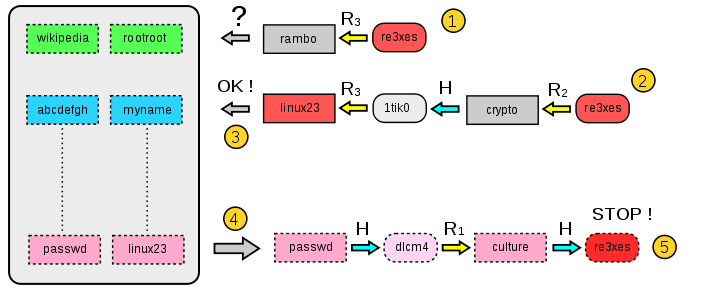
\includegraphics[scale=0.5]{crack}
\caption{彩虹表查表过程}
\label{fig:4.3}
\end{figure}

从图中我们看到需要破解的密钥为“re3xes”,第一步,将“re3xes”代入R函数,得到索引“rambo”,将此索引从每个彩虹链的末端开始对比;
第二步,若不匹配,则通过算法中的f函数\eqref{equ:10}进行遍历整条彩虹链,若在这条链表中没找到匹配的,则往后遍历表中的其他彩虹链;
第三步,当在链中找到匹配的索引后,记录该链表的首部索引;
第四步,通过第三步找到的索引,进行f函数计算得到产生目标密钥“re3xes”的明文“passwd”,并验证其正确性。
\subsection{假警分析}

\section{实验结构与分析}
\section{本章小结}
本章主要介绍了彩虹表算法的C++实现,主要包括彩虹表的预运算,即彩虹表的生成和利用彩虹表进行密钥破解。关键的程序代码可以参考附件。

\chapter{彩虹表算法的优化}
%\section{计算能力优化}
\section{基于CUDA并行计算优化}
密码破解主要的瓶颈在于现有的计算能力上,假如我们目前已经拥有量子计算机的处理能力,那么现有的所有的现代加密算法都是可以短时间内被破解的,所以我们要提升破解时间,最首要的办法就是对系统的计算能力进行优化,本文将提出两个优化方案,并实现了基于GPU的优化方案。
下面两张图为EWSA(Elcomsoft Wireless Security Auditor)对无线加密算法WPA/WPA2 PSK密钥破解的数据对比和Pyrit软件在GPU上加速后的数据对比。从图中数据可以看出采用了GPU加速后的
破解速度有很明显提升。
%\begin{figure}[!h]
%\begin{floatrow}
%\ffigbox{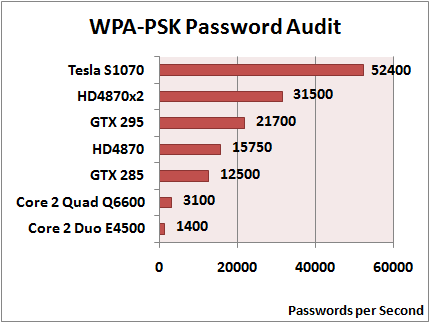
\includegraphics[scale=0.4]{ewsa}}{\caption{EWSA基于GPU加速破解WPA速度对比}}
%\ffigbox{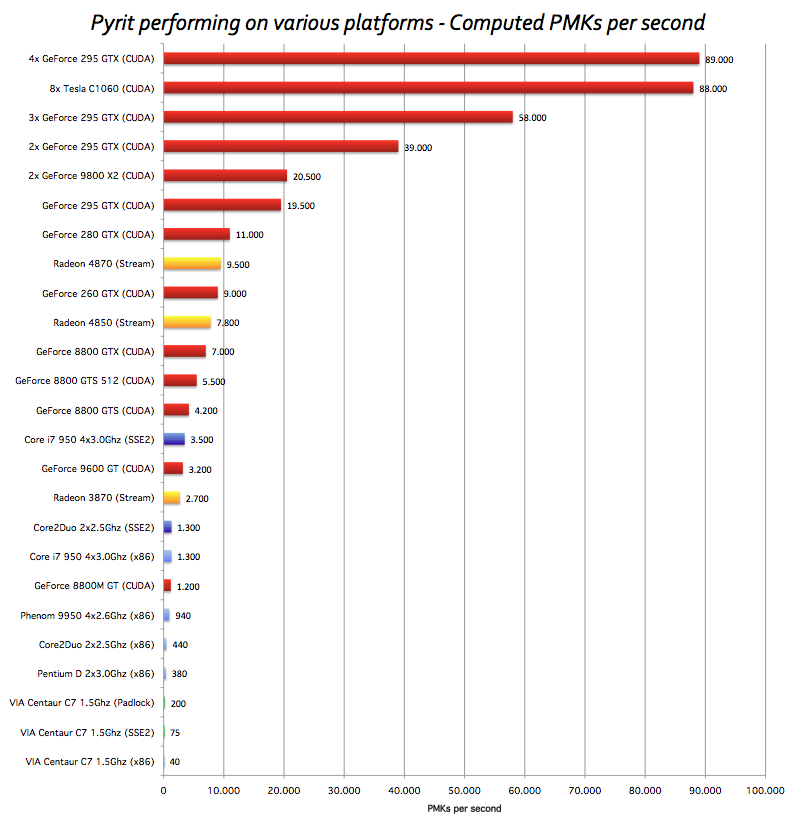
\includegraphics[scale=0.25]{pyrit}}{\caption{Pyrit基于CUDA性能测试}}
%\end{floatrow}
%\end{figure}
\begin{figure}[!ht]
\centering
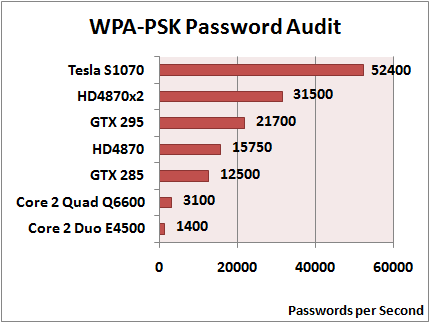
\includegraphics[scale=0.6]{ewsa}
\caption{EWSA基于GPU加速破解WPA密钥的速度对比}
%\label{fig:5.}
\end{figure}
\begin{figure}[!ht]
\centering
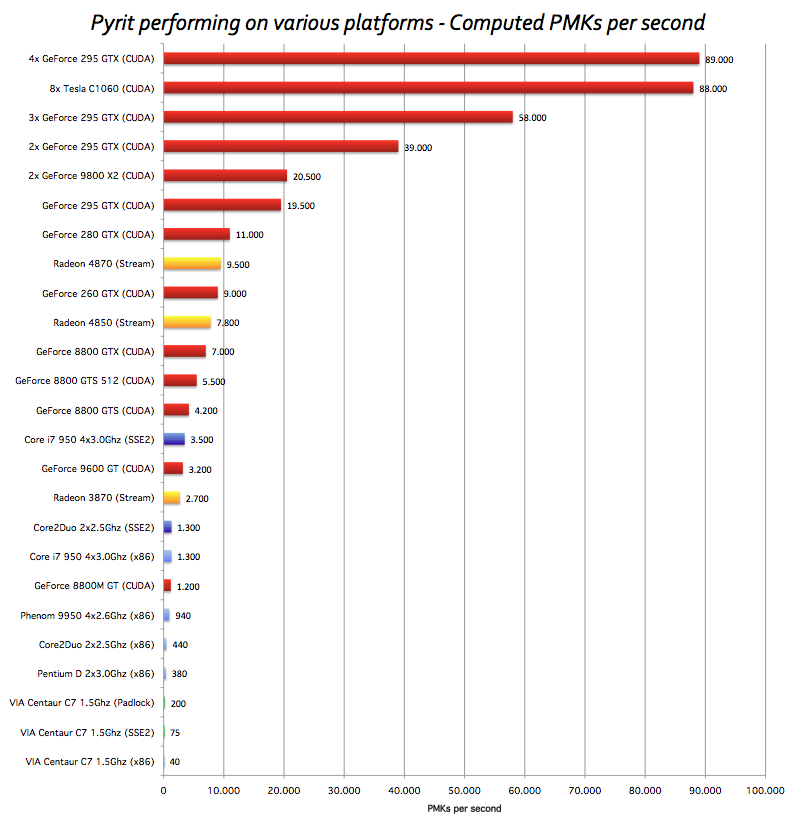
\includegraphics[scale=0.4]{pyrit}
\caption{Pyrit基于CUDA性能测试}
%\label{fig:5.1}
\end{figure}
基于GPU并行计算加快破解速度会受制与显卡本身的硬件条件限制,因为每个不同型号的显卡配备的显存、寄存器、线程调度数等等都是不一样的。如何在这些局限的硬件资源上合理分配,则是GPU程序设计的关键,也是性能提升的关键。例如如何控制在同一个线程组里的线程分支数、访问全局内存的顺序都是一些常用的优化代码的方法。在实际代码设计过程中,我们首先需要将计算任务并行化,把这些并行任务分配到线程上,再由这些线程组成线程块,这些线程块将会被线程管理器动态地分配到各个流处理器进行独立的并行计算。下面我们将从GPU的硬件特性和软件特性两方面进行优化,例如减小数据传输的开销、解决共享内存的访问冲突和降低条件分支的影响等等\cite{cuda01}。
Nvidia GPU不同构架的一些规格比较,见表\ref{tab:5.2}
\begin{longtable}{@{\extracolsep{\fill}}cccc}
\caption{三代GPU间的一些规格比较}\\\toprule[1pt]
\multicolumn{1}{c}{GPU} &
\multicolumn{1}{c}{G80} &
\multicolumn{1}{c}{GT200} &
\multicolumn{1}{c}{Fermi} \\\midrule
CUDA Cores & 128 & 240 & 512 \\
双浮点数计算能力 & 无 & 30FMA & 256FMA \\
单浮点数计算能力 & 128MAD & 240MAD  & 512FMA \\
特殊功能单元(SFUs)/SM & 2 & 2 & 4 \\
Warp调度器/SM & 1 & 1 & 2 \\
共享内存/SM & 16KB & 16KB & 可配置48KB/16KB \\
L1缓存/SM & 无 & 无 & 可配置16KB/48KB \\
L2缓存 & 无 & 无 & 768KB \\
ECC内存交验 & 不支持 & 不支持 & 支持 \\
并发内核数 & 无 & 无 & 最多16 \\
地址位宽 & 32b-bit & 32-bit & 64-bit \\
\bottomrule[1pt]
\label{tab:5.2}
\end{longtable}
\subsection{减小数据传输开销}
在目前的计算机体系结构中,像显卡这样的外设一般都是通过PCI-Express总线连接到北桥芯片,再通往CPU,这和主机内存共享与CPU传输带宽。当CUP与GPU的数据频繁交换时,这个数据传输的开销将会是程序性能主要瓶颈。因此我们的程序必须尽量地减少CPU与GPU的数据交换,通常的办法有在GPU中动态生成程序所需的数据,也可以采用异步调用,使数据传输和计算能基本同时进行。
\subsection{共享内存访问冲突}
在表\ref{tab:5.2}中我们可以看到每个SM都会拥有16KB的以上的共享内存,这块共享内存的作用是存储全局内存以外的数据,也可以作为块与块之间线程交换数据的媒介。它的访问速度比寄存器慢,但要比局部内存和全局内要快一些。如果不出现访问冲突,一个线程访问共享内存的速度几乎接近访问寄存器的速度。
图\ref{fig:5.11}Fermi构架的内存体系结构,除了拥有可配置的共享内存外,还有L1和L2的高速缓存。
\begin{figure}[!ht]
\centering
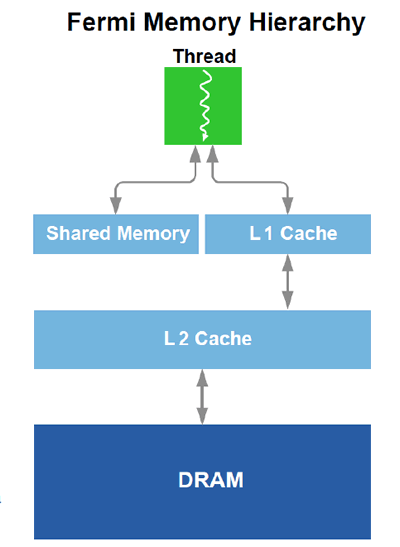
\includegraphics[scale=0.5]{fermi-memory}
\caption{Fermi构架的存储层次结构}
\label{fig:5.11}
\end{figure}
%\subsection{条件分支}
\subsection{核心配置优化}
核心程序的配置如块数、块内线程数都依赖核心代码本身,但仍然需要手工评估性能,排除大部分低效的配置。配置好块数和块内线程后,计算SM利用率,便可得到SM上活动Warp和最大Warp的比,通常我们也无需达到100\%。

首先,当线程请求的寄存器数大于块内最大寄存器,或者请求的寄存器、共享内
存超出了 SM 所提供的资源上限时,核心代码将无法正常启动。而一个块的寄存器占
用数 BR 可由下式计算得到:
\begin{equation}
Max(R*Max(T,32),\frac{R_{max}}{32})
\end{equation}
其中R表示核心请求的寄存器数,$R_{max}$表示 SM 所能提供的最大可用寄存器数,T 表
示用户指定的块内线程数。 以及Max(T,32)是为了保证一个SM应分配32个线程。
而一个块的共享内存总量则由静态共享内存、动态共享内存以及用于传递核心参数的
共享内存这三部共同组成。以上所请求的数值可通过向编译器指定 参数
(—ptxas-options=-v)的方式,在运行前获得并可作为资源估算的依据。对于寄存器
一项需要注意的是,double 以及 long long 类型的变量将占用两个 32 位寄存器。
结合核心请求的资源数,当我们确定了一次 CPU-GPU 交互之间参与计算的总线
程数 AS 后,块内线程数 BS 的确定将取决于$\frac{AS}{BS}$
个块是否能充分利用 GPU 提供的所
有 SM 的计算能力。首先,配置参数应指定至少与 SM 数相等的块数。其次,若 SM
只能分配得到一个块,则一旦块中的 Warps 均因为访存或线程同步等原因暂时挂起,
SM 将会因为没有活动块来掩盖访问延迟而处于空闲态。所以,通常应让 的数量
使得每个 SM 能有两个或两个以上的活动块,如此可以最多提升 50\%以上的性能。需
要注意的是,若希望有两个活动块,则需要 GPU 静态地拥有能满足两个块内所有线
程需求的资源。理论上,越多的活动块,越能够组成吞吐量更高的流水线,这也是我
们需要参照核心请求资源数,从而预先规划配置参数的原因。一般地一个格内至少应
有 100 个块,以适应 GPU 多级流水线的设计。除了要求有足够的块数,同样地块内
线程数也类似的方法。一般的块内线程数应是 Warp 大小(32)的倍数,以防止处理器
空转。理想情况下,一个块内的线程越多越好,但是仍然是由于资源的限制,越多的
线程,则每个线程所分配的寄存器、共享内存就越少,甚至会使得核心启动失败。一
般地,应有块内线程数大于 64,通常 192 或者 256 会是更好的选择,否则过少的线
程将很难掩盖块内 Warp 的访存延迟。

\subsection{指令级别优化}
这项优化工作一般是有GPU的编译器来作的,在CUDA中是有nvcc编译器来完成的。尽量使用低延迟的指令,对全局变量或寄存器以外的局部变量,尽量少用需要多次Load和Store的操作,需要减少循环操作的开销。以下为一些典型的优化方法:

1),我们知道 GPU 中诸如 mul,div 以及 rem 之类的指令,相较于
add,sub 以及位操作,其时钟延迟高出4-30倍之间,因而,需要尽可能不使用高延迟
指令或通过低延迟指令作等价的转换。如 CUDA2.3 的编译器,将32位的数组(uint
Array[size]) 的下标操作翻译为$Array+index*4$,而等价的低延迟操作为
$Array+index<<2$。此情况可通过保留Array的类型的方法,来克服由强制转换带来的
编译器优化困难。

2),对于全局变量或难以寄存器外的局部变量,应尽量减少$+=,*=$等需要多次
Load 和 Store 的操作,通常应将相应变量放入寄存器或者共享存储。
3),对于循环操作,CUDA 提供了$\#pragma \quad unroll$关键字用于简单循环的展开
以减少分支和循环本身的开销。但是当需要对循环展开时,仍然需要仔细观察循环体
本身,并在资源使用、局部性以及上下文相关性等方面做权衡。一般的简单循环编译
器会自动展开,特别是当循环体中的指令数接近于循环外层所需要指令时通常建义展
开,而当循环次数较大时则只能由开发者显式地指定循环展开层数。同时我们也应注
意到,当循环体中的复杂操作前后相关性较大(例如前一操作的结果是后一操作输入)
或者后一循环依赖于上一个循环时,展开效果将并不明显。因为展开后的代码也很难
利用 GPU 中的流水线处理机制。但无论采用那种方式,都应该检查编译后的 PTX 是否
合理,尤其是寄存器使用情况、跳转指令条数和位置等,以防止编译器作出错误的优
化判断。
\subsection{存储合并访问}
从文献\cite{cuda05}可知,SM会以时间片轮询的方式逐个调度每个Warp。各个 SM 一次只需要足够的资源以运行运行 32 个线程(通常块内线程数要远大于 32),其中的 8 个 SP 将分 4 个及其周期的时间偏离所有的线程(我们假设此处的指令为大多数可在一个周期内完成简单指令)。
当 SM 执行一条访存指令时,它首先会发出一条访存请求,并随机转向下一个就绪 Warp,而当前 Warp 将被挂起直到数据访问完成,才能再次进入就绪态并被等待属于它的时间片。理想的情况下,该 Warp 内的访存请求没有冲突,则该请求可在一个访存事务内完成。然而,事实上是否能在一个事务中结束访问,是严重依赖于 Warp内每个线程所访问存储的地址是否可合并这个事实的(Coalesced MemoryAccesses)。简单地讲,如果每个线程的访存地址是连续的,则所有 Warp 内的请求可以合并为一
个访存事务,否则将可能产生多个事务并导致该 Warp 需要更多的等待时间\cite{cuda02}。
\subsection{基于CUDA的云计算平台}
云计算是网格计算、分布式计算、并行计算、效用计算、网络存储、虚拟化、负载均衡等传统计算机和网络技术发展融合的产物。在\cite{word}一文中使用了Hadoop分布式集群优化彩虹表算法,实际上Hadoop也可以称之为一种云平台。我们也可以设计一个基于GPU加速的云计算平台,通过云平台的计算能力提升彩虹表的预运算和破解的速度。
亚马逊EC2就是这样的一个平台,它可以让用户按照自己的硬件需求租用计算机来获取计算能力。
\section{存储优化}
对于时空折中算法而言,除了要对时间进行优化,还有对空间进行优化,在不增加(或增加少量)时间代价的前提,如何减小空间代价,这就需要我们对系统进行存储优化,因为时空折中算法的性能随着存储空间的减少而降低。我们将从两方面进行改进。第一,针对存储文件本身进行优化,也就是彩虹表文件,我们将设计一个新型的彩虹表存储结构体,减少彩虹表的磁盘存储空间,缩小系统读取文件的时间,从而提升破解的速度;第二,优化存储系统,如采用适合大文件的文件系统,采用快速的物理存储设备等方面提升读取速度。
\subsection{新型彩虹表文件}
从上一章彩虹表磁盘空间占用公式\eqref{equ:4.2}可知,想要覆盖更大的密钥空间要么增加彩虹链数或者彩虹表的张数,这都回产生庞大的彩虹表文件,可能会达到几百个GB,甚至上TB的文件,这将会增加大量的文件读取时间和磁盘空间,因此对表的存储结构进行优化将十分有必要。
我们将新设计的彩虹链,在以前的存储结构中我们是使用了一个64比特的非负整形变量定义开始节点,而在实际当中,我们并没有必要全部使用这64比特的数据来存储它,实际上只要能保证彩虹链的初始节点是随机地来自密钥空间N就可以。在第四章中的ntlm的彩虹表中,我们只定义了26比特的开始节点和30比特的末端节点,这样一条彩虹链所占用的字节数为7Bytes。代入公式\eqref{equ:4.2}可以得到一张优化后的表的大小为448MB,优化了56.25\%。这样大大减小系统的存储空间和读取文件的时间。
\begin{figure}[!ht]
\centering
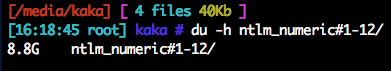
\includegraphics[scale=0.7]{5-1.png}
\caption{优化后彩虹表的空间大小}
\label{fig:5.1}
\end{figure}

新的彩虹链的数据结构实现如下,在以后的测试实验中,我们将都采用这种优化过的彩虹表。
\begin{lstlisting}
struct RTCFileHeader
{
    unsigned int   uVersion;    
    unsigned short uIndexSBits; 
    unsigned short uIndexEBits; 
    uint64         uIndexSMin;
    uint64         uIndexEMin;
    uint64         uIndexEInterval;
};
\end{lstlisting}
\subsection{文件系统的优化}
在存储上,除了对表的大小进行优化,还可以对系统的储存架构进行优化。在文件系统上,我们采用先进的XFS文件系统,XFS是由Silico Graphics,Inc.于90年代初开发的,它采用了优化算法,对查询分配存储空间非常快,可以支持上百万T字节的存储空间,特别是对大文件的支持表现相当出众;XFS采用B+树结构保证文件系统可以快速搜索于空间分配;XFS几乎以接近裸设备I/O的性能存储数据,在单个文件系统测试种,其吞吐量可高达7GB每秒,对单个文件的读写操作,其吞吐量可达4GB每秒。基于XFS以上特性,正符合彩虹表多个大文件读取的特点,下图为XFS与EXT3、EXT4的性能比较:
%\begin{figure}[!h]
%\begin{floatrow}
%\ffigbox{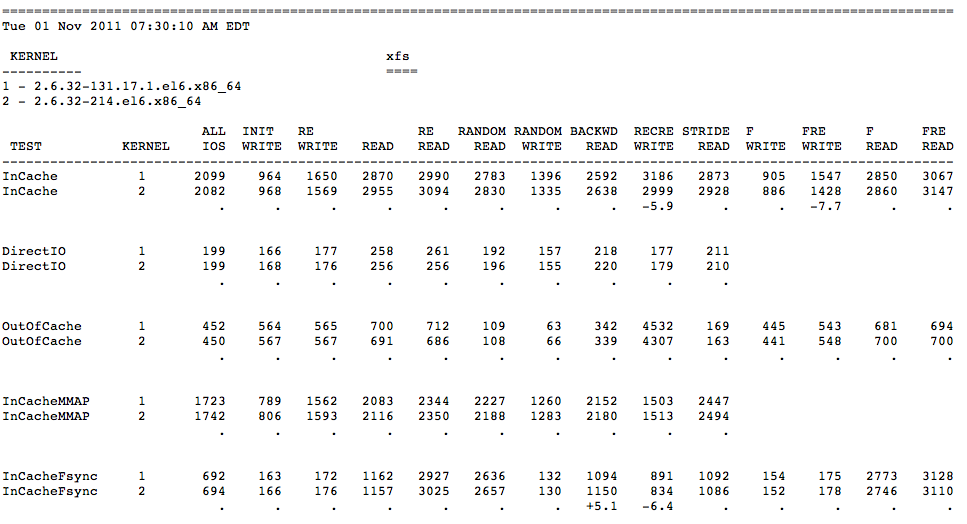
\includegraphics[scale=0.2]{5-2}}{\caption{XFS文件系统性能测试}}
%\ffigbox{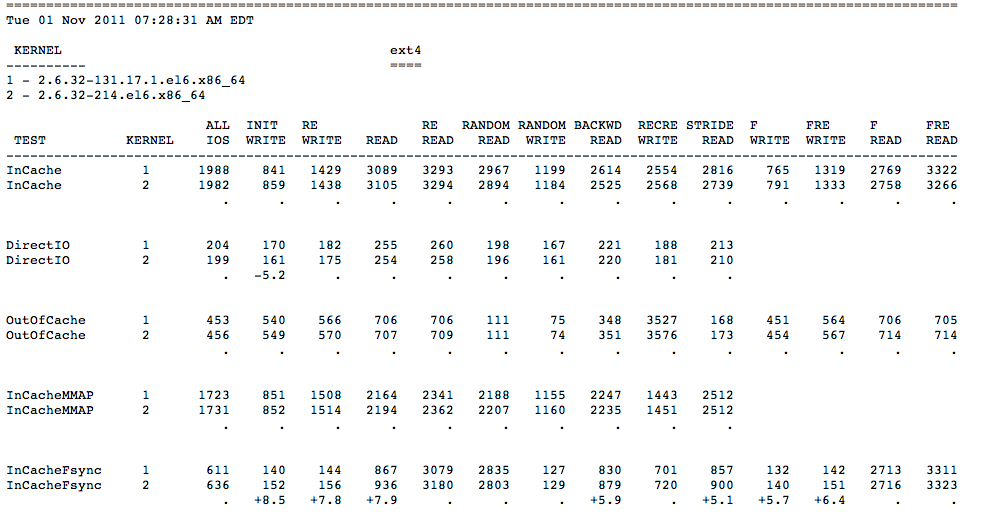
\includegraphics[scale=0.2]{5-3}}{\caption{EXT4文件系统行性能测试}}
%\end{floatrow}
%\end{figure}
\begin{figure}[!ht]
\centering
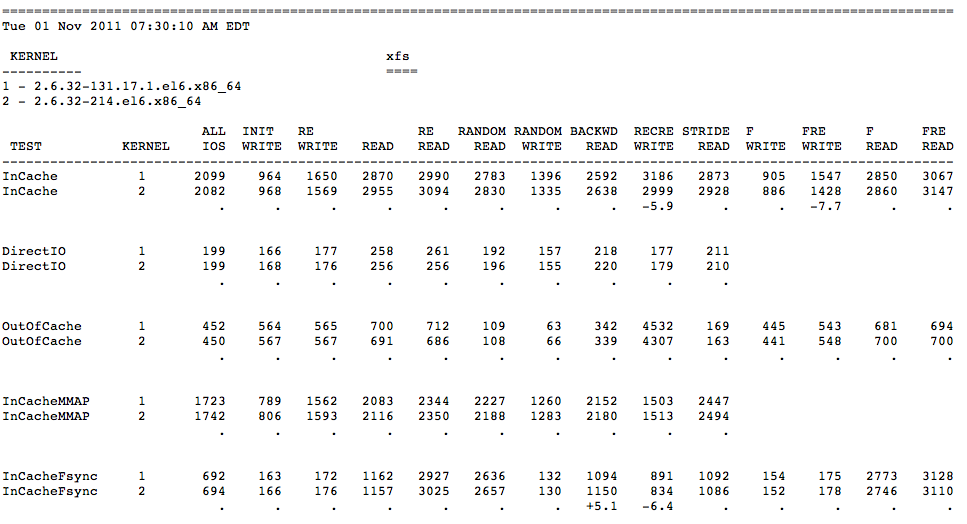
\includegraphics[scale=0.4]{5-2.png}
\caption{XFS性能测试}
\label{fig:5.2}
\end{figure}
\begin{figure}[!ht]
\centering
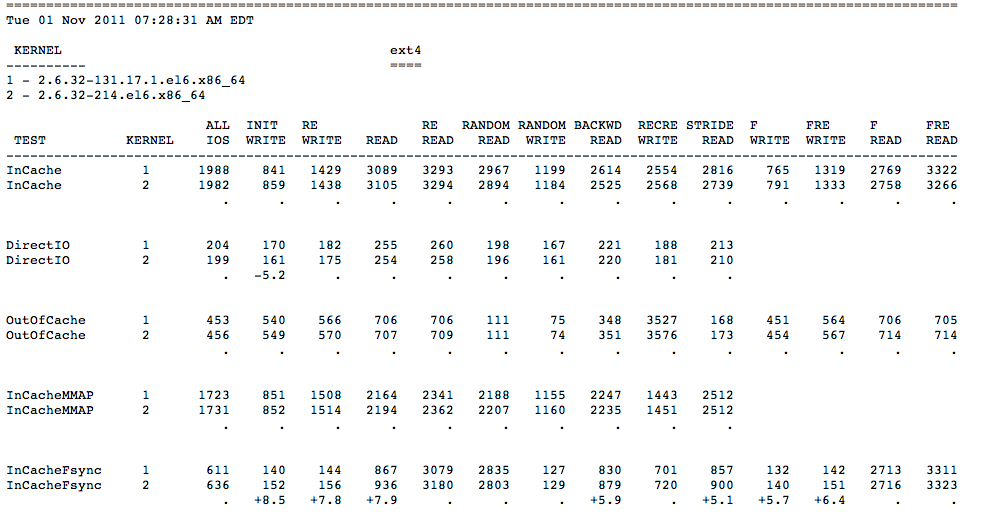
\includegraphics[scale=0.4]{5-3.png}
\caption{EXT4性能测试}
\end{figure}
\begin{figure}[!ht]
\centering
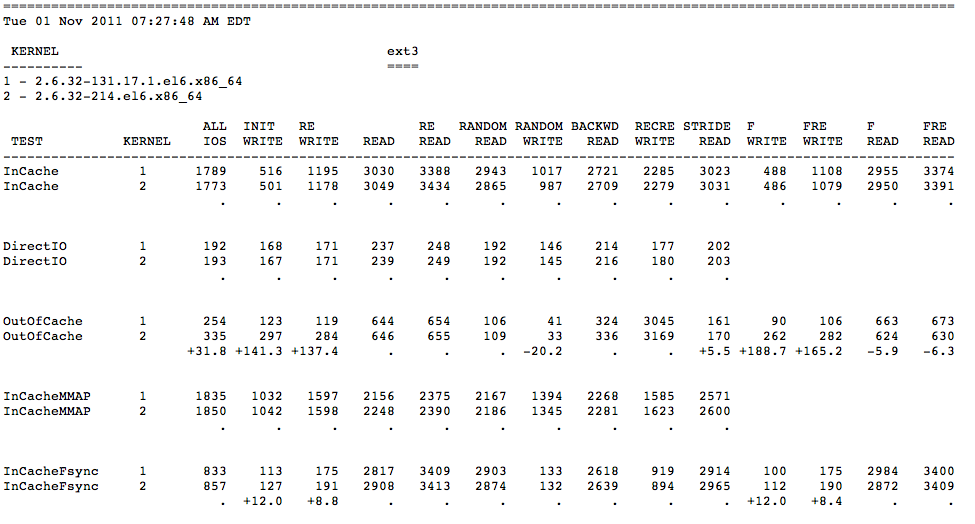
\includegraphics[scale=0.4]{5-4.png}
\caption{EXT3性能测试}
\end{figure}
从这上面两组性能测试数据我们可以看出XFS在大多数的的选项上要优于EXT4文件系统,特别是在大文件的读取上。
\subsection{存储技术的优化}
目前的存储技术主要分为三大类:直接附加存储、网络附加存储和SAN存储方式。
直接附加存储方式与我们普通PC的存储构架一样,外部的存储设备都是直接连接在服务器的内部总线上,是整个服务器结构的一部分。
网络附加存储方式则全面改进了以前低效的DAS存储方式。它采用独立于服务器,单独为网络数据存储而开发的一种文件服务器来连接所存储设备,自形成一个网络。这样数据存储就不再是服务器的附属,而是作为独立网络节点而存在于网络之中,可由所有的网络用户共享。
SAN存储方式创造了存储的网络化。存储网络化顺应了计算机服务器体系结构网络化的趋势。SAN的支撑技术是光纤通道(FC Fiber Channel)技术。它是ANSI为网络和通道I/O接口建立的一个标准集成。FC技术支持HIPPI、IPI、SCSI、IP、ATM等多种高级协议,其最大特性是将网络和设备的通信协议与传输物理介质隔离开,这样多种协议可在同一个物理连接上同时传送。

我们还可以采用iSCSI网络存储结构,iSCSI技术一种优IBM公司研究开发的,是一种新存储技术,可是实现在IP网络上运行SCSI协议,使其能在高速千兆或万兆以太网上进行网络传输。再加上FCoE技术,可以达到几Gb/s的存储速度。

接着是对存储硬件升级,这里我们主要升级的是硬盘,下表\ref{tab:5.1}是我们对不同配置硬盘的读速度进行数据对比,从表中可以明显看出使用SSD硬盘RAID0阵列后,读取速度将比一块7200转的硬盘提升了10倍,这将大大缩小破解的实际时间。最后的需要升级的系统内存,我们知道在计算机存储体系结构中,内存的读取速度要比硬盘快上许多倍,在Linux系统上内存以/dev/shm/设备呈现给用户,用户可以对次进行读写操作。
\begin{longtable}{@{\extracolsep{\fill}}ccc}
\caption{各种存储系统读速度对比数据}\\\toprule[1pt]
\multicolumn{1}{c}{硬盘配置} &
\multicolumn{1}{c}{读速度(hdparm -t)} &
\multicolumn{1}{c}{索引速度} \\\midrule
1x Maxtor 6B250S0 7200 RPM & 54MB/s & 640h/s \\
6x Seagate 7200 RPM (RAID6) & 390MB/s & 4375h/s \\
2x APPLE SSD SM128C (RAID0) & 522MB/s & 6120h/s \\
\bottomrule[1pt]
\label{tab:5.1}
\end{longtable}
在HP\quad DL580g7服务器上配置有16GB的内存,而我们实验所用的彩虹表一共占用磁盘空间8.8GB,我们把磁盘上的文件目录挂载到tmpfs文件系统上,
执行命令$“mount\quad -t\quad tmpfs\quad -o\quad size=100\%\quad /test”$,然后关闭交换分区$“swapoff\quad -a”$。
为了消除缓存的影响,我们清空所有虚拟内存的缓存$“echo\quad 3\quad >\quad /proc/sys/vm/drop\_caches”$。
\begin{figure}[!ht]
\centering
\includegraphics[scale=0.7]{disk}
\caption{从硬盘读取的效率}
\end{figure}
\begin{figure}[!ht]
\centering
\includegraphics[scale=0.7]{memory}
\caption{直接从内存读取}
\end{figure}

从上面实验结果可以看出,使用硬盘的读取时间为11.14s,预先把文件写入内存后,直接读取内存的时间为2.49s,当然这里面还有内存缺页的损失,所以只提升了4.47倍,但是可以验证了这一设想的正确性。
\section{算法结构优化}
密钥明文字符集被预计算成hash密文并和明文成对地储存在彩虹链中,如果要破解的hash密文在我们之前生成好的彩虹链中,则破解成功,反之破解失败。彩虹链存储的“明文-密文”对数量随着链表长度(t)的增加而增加,然而这些彩虹链会产生冲突,主要由于减约函数并不是一一对应的。图\ref{fig:5.5}示意了冲突的过程,最后这两条链表会合并成一条。
\begin{figure}[!ht]
\centering
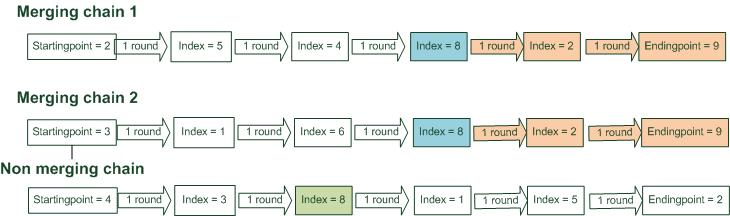
\includegraphics[scale=0.7]{5-5}
\caption{链表合并过程示意图}
\label{fig:5.5}
\end{figure}

无冲突的彩虹链个数会随着彩虹表的长度增加而减少,根据公式\eqref{equ:3.13},利用matlab软件我们可以得到关系图\ref{fig:5.6}。
\begin{figure}[!ht]
\centering
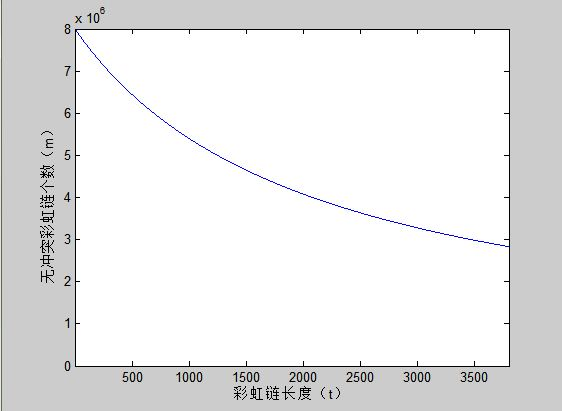
\includegraphics[scale=0.5]{5-6}
\caption{无冲突链表数-链表长度关系}
\label{fig:5.6}
\end{figure}

接着我们来分析表的张数(参数l)对破解成功概率的影响,我们把破解成功率公式\eqref{equ:3.13}在matlab下的实现函数为:\\
demo\_advantage\_of\_multiple\_table(),具体的函数实现可以参考附录A1.2。我们用不同的曲线表示当硬盘空间增大的情况下,破解的成功概率会随之增加,下图中有5条曲线,分别表示彩虹表张数为1\~5时,破解的成功率和硬盘空间之间的关系,放大后,我们可以看出彩虹表的张数越多,曲线越快接近100\%,也就是在其他参数不变的情况下,增加参数l(彩虹表张数),可以得到越高破解成功概率;但也不是生成的彩虹表张数越多越好,当随着彩虹表的增加,我们需要在存储空间也就越大,这样会破解实际所消耗的时间就会增加,反而适得其反,所以时空折中算法的精髓就在于对时间和空间的代价进行不断地平衡,找出一个折中的代价。
\begin{figure}[!h]
\begin{floatrow}
\ffigbox{\caption{5张彩虹表的破解成功率}}{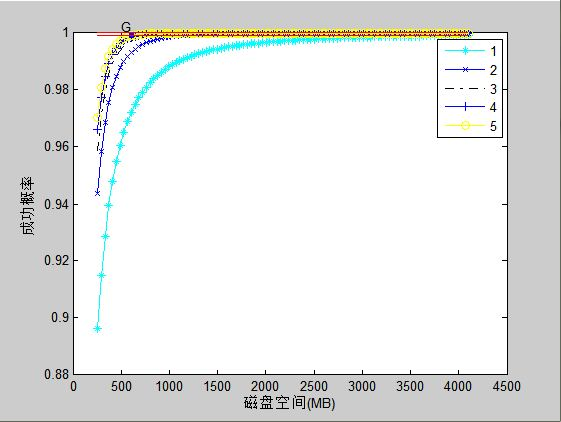
\includegraphics[scale=0.35]{5-7}}
\ffigbox{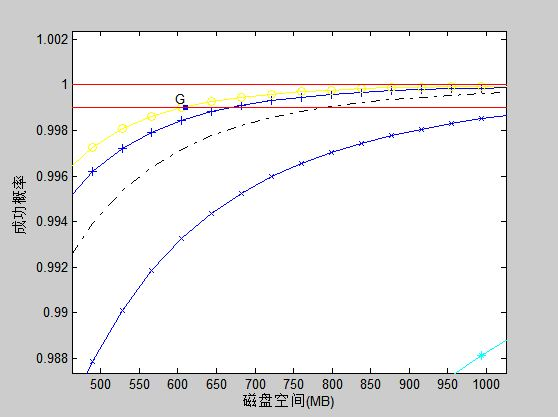
\includegraphics[scale=0.35]{5-8}}{\caption{5张彩虹表的破解成功率(放大)}}
\end{floatrow}
%\label{fig:5.7}
\end{figure}
\begin{figure}[!h]
\begin{floatrow}
\ffigbox{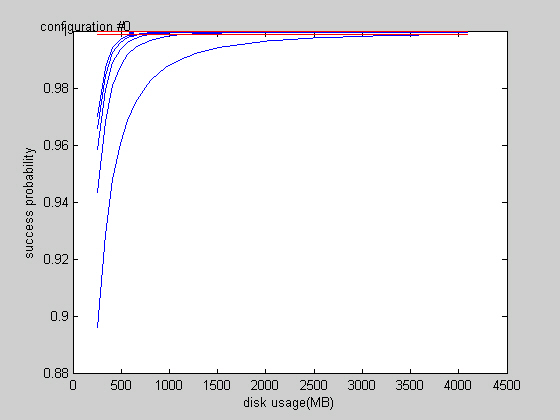
\includegraphics[scale=0.35]{5-9}}{\caption{总表空间大小-成功率关系图}}
\ffigbox{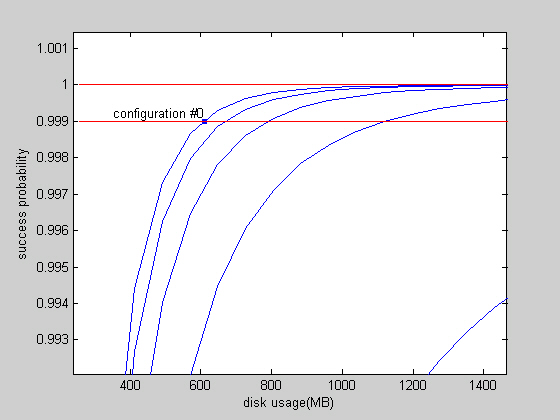
\includegraphics[scale=0.35]{5-10}}{\caption{总表空间大小-成功率关系图(放大)}}
\end{floatrow}
\end{figure}
\clearpage
\section{实验结果与分析}
实验所用的测试平台见下表\ref{tab:5.3}:
\begin{longtable}{@{\extracolsep{\fill}}cc}
\caption{实验数据测试平台配置}\\\toprule[1pt]
\multicolumn{1}{c}{CPU} & \multicolumn{1}{c}{Intel Core i7-920 OC 4.0GHz (EIST/C1E off)} \\\hline
主板 & Asustek Rampage II GeneIntel X58芯片 \\\hline
显卡 & GeForce GTX 480 1536MB(Core/Shader/memory:700/1401/1848MHz) \\\hline
内存 & GSKILL F3-12800CL9T OC DDR3-1600 2G*3 \\\hline
硬盘 & 2x Intel 120G SSD SM128C (RAID0) \\\hline
电源 &  CougarGX 900W  \\
\bottomrule[1pt]
\label{tab:5.3}
\end{longtable}
\subsection{破解速度实验对比}
实验方法是通过采用上述优化方法和技术,对SHA-1 、MD5和NTLM三种Hash加密算法进行实验,我们规定密钥的字符集范围(字符集对照表参见附录\ref{cha:a_c}),密钥长度,限定成功率在99.9\%以上,主要从破解时间方面针对优化前和优化后的实验数据进行对比。

在这里需要说明的是破解的时间主要分为对彩虹表文件的读取时间和密钥查表破解的时间。对彩虹表文件的读取时间主要优化方法和技术参见本章的存储优化一节,上文已经给出了基本的实验对比数据,就不在这里赘述,我们只对比最后的实际破解时间。
所有实验只针对1条Hash密文进行破解,每组彩虹表破解3次。

SHA1破解实验,破解速度提升了5.88倍,详细实验数据参考下表\ref{tab:5.5}:
\begin{longtable}{@{\extracolsep{\fill}}ccccc}
\caption{SHA1破解实验数据对比}\\\toprule[1pt]
\multicolumn{1}{c}{字符集} &
\multicolumn{1}{c}{密钥长度} &
\multicolumn{1}{c}{成功率} &
\multicolumn{1}{c}{优化前破解时间(秒)}&
\multicolumn{1}{c}{优化后破解时间(秒)}\\\midrule
\endfirsthead
\caption[]{SHA1破解实验数据对比(续)}\\
\multicolumn{5}{r}{\footnotesize 接上页}\\
\toprule[1pt]
\multicolumn{1}{c}{字符集} &
\multicolumn{1}{c}{密钥长度} &
\multicolumn{1}{c}{成功率} &
\multicolumn{1}{c}{优化前破解时间(秒)}&
\multicolumn{1}{c}{优化后破解时间(秒)}\\\endhead
numeric & 1~12 & 99.9\% & 27.54 & 4.78 \\
numeric & 1~12 & 99.9\% & 23.32 & 4.04 \\
numeric & 1~12 & 99.9\% & 36.21 & 5.98 \\\hline
loweralpha & 1~9 & 99.9\% & 21.08 & 6.76 \\
loweralpha & 1~9 & 99.9\% & 19.65 & 5.88 \\
loweralpha & 1~9 & 99.9\% & 30.18 & 8.90 \\\hline

\bottomrule[1pt]
\label{tab:5.5}
\end{longtable}
MD5破解实验,破解速度提升了6.3倍,详细实验数据参考下表\ref{tab:5.6}:
\begin{longtable}{@{\extracolsep{\fill}}ccccc}
\caption{MD5破解实验数据对比}\\\toprule[1pt]
\multicolumn{1}{c}{字符集} &
\multicolumn{1}{c}{密钥长度} &
\multicolumn{1}{c}{成功率} &
\multicolumn{1}{c}{优化前破解时间(秒)}&
\multicolumn{1}{c}{优化后破解时间(秒)}\\\midrule
ascii-32-95 & 1~7 & 99.9\% & 372.33 & 69.47 \\
ascii-32-95 & 1~7 & 99.9\% & 487.26 & 54.90 \\
ascii-32-95 & 1~7 & 99.9\% & 432.98 & 96.22 \\\hline
loweralpha & 1~9 & 99.9\% & 41.92 & 30.09 \\
loweralpha & 1~9 & 99.9\% & 76.22 & 12.56 \\
loweralpha & 1~9 & 99.9\% & 25.46 & 31.18 \\
\bottomrule[1pt]
\label{tab:5.6}
\end{longtable}
NTLM破解实验,破解速度提升了1.77倍,详细实验数据参考下表\ref{tab:5.7}:
\begin{longtable}{@{\extracolsep{\fill}}ccccc}
\caption{NTLM破解实验数据对比}\\\toprule[1pt]
\multicolumn{1}{c}{字符集} &
\multicolumn{1}{c}{密钥长度} &
\multicolumn{1}{c}{成功率} &
\multicolumn{1}{c}{优化前破解时间(秒)}&
\multicolumn{1}{c}{优化后破解时间(秒)}\\\midrule
numeric & 1~12 & 99.9\% & 8.32 & 7.43 \\
numeric & 1~12 & 99.9\% & 10.76 & 6.90 \\
numeric & 1~12 & 99.9\% & 5.45 & 2.08 \\\hline
loweralpha & 1~9 & 99.9\% & 17.25 & 4.32 \\
loweralpha & 1~9 & 99.9\% & 12.87 & 3.66 \\
loweralpha & 1~9 & 99.9\% & 12.44 & 10.71 \\
\bottomrule[1pt]
\label{tab:5.7}
\end{longtable}
\subsection{与等规模的旧表的性能对比实验}
在这个实验中,我们采用新型的彩虹表结构生成彩虹表文件,选择针对Hash算法性能性能较好的26比特和30比特,在保证单张新表和原始彩虹表存储空间代价M相等的前提下,通过比较l张新表与相应的单表在破解时间T、假警数量和成功率P之间的关系,验证了5.2节中的存储优化的效果,并且从另外一方面观察彩虹表的存储空间大小对破解成功率与假警数量变化的关系。
\begin{longtable}{@{\extracolsep{\fill}}ccccccccccc}
\caption{新表与等空间的单张彩虹表的性能对比}\\\toprule[1pt]
\multicolumn{1}{c}{瘦} & \multicolumn{5}{c}{新表} & \multicolumn{5}{c}{单张彩虹表} \\
\multicolumn{1}{c}{表} \\
\multicolumn{1}{c}{张} & \multicolumn{1}{c}{Hellman} & \multicolumn{1}{c}{本文} & \multicolumn{1}{c}{实际} & \multicolumn{1}{c}{T(s)} & \multicolumn{1}{c}{P} &
\multicolumn{1}{c}{Hellman} & \multicolumn{1}{c}{本文} & \multicolumn{1}{c}{实际} & \multicolumn{1}{c}{T(s)} & \multicolumn{1}{c}{P} \\
\multicolumn{1}{c}{数} & \multicolumn{1}{c}{FA数} & \multicolumn{1}{c}{FA数} & \multicolumn{1}{c}{FA数} &  &  &
\multicolumn{1}{c}{FA数} & \multicolumn{1}{c}{FA数} & \multicolumn{1}{c}{FA数} & &  \\\midrule
1 & 512  & 462  & 480  & 2.1 & 40.3\% & 409  & 380  & 370  & 2.0 & 44\%    \\
2 & 1024 & 843  & 920  & 2.8 & 49.8\% & 818  & 722  & 702  & 3.1 & 53\%   \\
3 & 1536 & 1120 & 1332 & 3.4 & 54.7\% & 1346 & 1120 & 1023 & 3.3 & 59\%  \\
4 & 2048 & 1873 & 1587 & 4.3 & 64.6\% & 1638 & 1380 & 1287 & 4.4 & 64\%  \\
5 & 2560 & 2011 & 2143 & 4.6 & 75.2\% & 2280 & 2098 & 2100 & 4.7 & 74\% \\
6 & 3072 & 2101 & 2248 & 5.8 & 89.4\% & 2460 & 2287 & 2309 & 5.6 & 85\%    \\
7 & 3584 & 2239 & 2478 & 5.7 & 96.8\% & 2876 & 2389 & 2408 & 6.1 & 90\% \\
8 & 4096 & 2489 & 2998 & 6.8 & 99.9\% & 3287 & 2502 & 2512 & 6.3 & 94\%  \\
\bottomrule[1pt]
\label{tab:5.7}
\end{longtable}

\section{本章小结}
本章对从计算能力到存储和彩虹表算法结构三方面进行优化和实现。在计算能力上我们提出了基于CUDA优化方法,并实现了CUDA GPU方案,从实际实验结果验证了这一设计方案;在存储系统上,我们提出了采用新型的彩虹表结构体,减少了彩虹表的磁盘存储空间,优化升级了物理的存储设备,在破解时间上得到了很好的提升;在彩虹表算法参数上,我们进行数据分析,优化了算法的参数。



\chapter{本文总结与展望}
\section{总结}
\section{展望}


%Reference
%\bibliographystyle{plain} \bibliography{reference}
\bibliographystyle{unsrt} \bibliography{reference}
\nocite{*}
\addcontentsline{toc}{chapter}{参考文献} 
\end{document}

